\documentclass[preprint]{sigplanconf}
\usepackage{amsmath,amssymb,amsthm}
\usepackage{color,graphicx,subfigure}
\usepackage{algpseudocode}
\algtext*{EndWhile}% Remove "end while" text
\algtext*{EndIf}% Remove "end if" text
\algtext*{EndFor}% Remove "end for" text
\usepackage{qtree}
\usepackage{epsfig,epstopdf}
\usepackage{multirow}
\usepackage{listings}
\usepackage{url}

\newcommand{\shrink}{\vspace*{-2ex}}

\newcommand{\TODO}[1]{\vspace*{2mm}\textcolor{red}{\fbox{TODO: #1}}\vspace*{2mm}}
\newcommand{\XJ}[1]{\textcolor{red}{[XJ: #1]}}
\newcommand{\KZ}[1]{\textcolor{blue}{[KZ: #1]}}
\newcommand{\RY}[1]{\textcolor{blue}{[RY: #1]}}

\newcommand{\nat}{\mathbb{N}}

\newcommand{\cm}{\mathbf{cm}}
\newcommand{\cu}{\mathbf{cu}}
\newcommand{\exit}{\mathbf{exit}}
\newcommand{\To}{\longrightarrow}
\newcommand{\computes}{\To_p}
\newcommand{\exiting}{\mathbf{exiting}}
\newcommand{\exited}{\mathbf{exited}}

\newcommand{\In}{\mathbf{in}}
\newcommand{\Out}{\mathbf{out}}
\newcommand{\Rd}{\mathbf{rd}}

\newcommand{\dm}{\mathcal{DM}}
\newcommand{\alltype}{\mathcal{T}}
\newcommand{\allop}{\mathcal{P}}
\newcommand{\allstore}{\mathcal{D}}

\newcommand{\typeof}[1]{\tau\ldbrack #1\rdbrack}

\newcommand{\ldbrack}{[\hspace{-0.5mm}[}
\newcommand{\rdbrack}{]\hspace{-0.5mm}]}
\newcommand{\lbb}{\{\hspace{-0.7mm}|}
\newcommand{\rbb}{|\hspace{-0.7mm}\}}

\newcommand{\compact}[1]{\!\!#1\!}
\newcommand{\bk}{\hspace{-1mm}}

\newtheorem{theorem}{Theorem}
\newtheorem{lemma}{Lemma}
\newtheorem{proposition}{Proposition}
\newtheorem{corollary}{Corollary}
\newtheorem{definition}{Definition}
\newtheorem{property}{Property}
\newtheorem{axiom}{Axiom}
\newtheorem{example}{Example}

\newcommand{\figref}[1]{Figure \ref{#1}}
\newcommand{\tabref}[1]{Table \ref{#1}}
\newcommand{\eqnref}[1]{Eq. (\ref{#1})}

\newcommand{\nl}{\vspace*{3mm}}

% \makeatletter
%  \let\@copyrightspace\relax
% \makeatother

\lstset{
  captionpos=b,
  tabsize=2,
  % numbers=left,
  % numberstyle=\tiny,
  % numbersep=5pt,
  breaklines=true,
  showstringspaces=true,
  basicstyle=\scriptsize\ttfamily,
  frame=none,
  emph={label},
  escapechar=| % Escape to LaTeX between |...|
}

\renewcommand{\shrink}{\vspace*{-2ex}}

\title{Speculative Nondeterminism}
\authorinfo{}{}{} % enable double-blind reviewing

\begin{document}

\maketitle

\begin{abstract}
We propose a new programmable concurrency control framework called
speculative nondeterminism for real time,
``open'' and distributed agents. 
%By open, we mean the agent programs
%are independent and are not necessarily constrained to operate
%in a particular fashion, and they may join the system at arbitrary times.
In this framework, dynamic and concurrent agent programs 
affect each other through a centralized store which represents shared resources.
%There is no direct communication among the agents.
%Because a sequential agent maybe blocked due to resource constraints
%in the store,
Our framework has novel programming constructs which
allows an agent to speculate against the future by multiple
exclusive choices that encode different strategies to achieve its goals.
The agent can make multiple choices which execute together but in isolation,
thus, there is a combinatorial effect through the joint interaction.
% The choices from the same agent execute in isolation but the choices from
% different agents interact through the store in a combinatorial fashion.
Unlike other concurrency frameworks, speculation models many potential
outcomes and thus improves the chances of an agent reaching a desired outcome.
% The benefit of speculation is that unlike other concurrency frameworks,
% the combinatorial-choice models more possibilities and
% improves the chances of successful outcomes for any participating agent.
Each possibility is represented by a ``virtual world.''
Agents operate in the virtual worlds created by the system,
the framework provides mechanisms for agents which have reached their
objective but yet are represented by multiple possible worlds to cleanly
exit. We also provide mechanisms to reduce the possibilities where an
agent can commit to certainly possibilities and give up on others, but
this is rather different from conventional committed choice.
% further allows the agents who have achieved their objectives
% in all existing worlds to exit and return to reality without delay.
% The choices from the same agent are meant to be executed in
% isolation from each other because they may update the store in different ways.
% Only one successful choice becomes the eventual reality. When multiple
% agents each specifies some choices, the system creates
% many stores and thus runtime environments to represent the
% different combinations of choices. We argue that combinatorial choices
% improve the likelihood of successful program completion and
% thus improve the overall system throughput.
% This is achieved with the programmable ``exit'' and ``commit'' operators
% where ``exit'' indicates that the agent program terminates and
% ``commit'' specifies when and where in the program agent wants to commit 
% to a particular choice and remove all other worlds (possibilities) associated
% with the other choice. This mechanism also controls the space of choices 
% and reclaims valuable computation resources to make the system practical. 
This paper presents the design, operational semantics of 
speculative nondeterminism, small but practical examples illustrating
the use of the language and experimental results of a prototype.
% demonstrates a prototype implementation of 
% the framework along with extensive evaluation results.
\end{abstract}

\keywords
speculation, concurrency, nondeterminism, agents

%\IEEEraisesectionheading{
% %\IEEEraisesectionheading{
% %\IEEEraisesectionheading{
% \input{intro}
\section{Introduction}\label{sec:intro}
 %}
% \section{Introduction}\label{sec:intro}

% \begin{enumerate}
% \item Motivation: application scenarios (with 1-2 running examples);
% \item Characteristics of the data sources and their challenges;
% \item Briefly introduce previous approaches to extract information 
% from images including setting the document zone, and their limitations.
% \item General flow of our approach (may give a diagram here)
% \end{enumerate}
% scenary

Due to ever evolving hardware and software, many medical images
such as electro-cardio graphs (ECGs), X-ray or ultrasound images  
are directly printed and stored in hard copy formats. 
% \KZ{Insert 4 example images here.}
%Examples are shown in \figref{fig:medicalImages}. 
% These images often contain a mix of graphics and text, which
% include parameter settings of the hardware, test measurements or simple
% diagnosis. 
These images often contain a mix of graphics and text, which 
include technical settings of the hardware used, test measurements or simple diagnoses.
Recently, there has been a growing demand for digitizing such 
medical information from paper media sources, especially legacy ones, or patients who want to keep track of these documents by themselves digitally. 
Apart from scanning the graphics into a digital format, extracting 
the semi-structured textual information is also an important part of
building electronic medical records for patients. 

%\begin{figure}[!htb]
%\centering
%\subfloat[ECG]{
%\label{fig:medicalimage:ecg}
%
\epsfig{file=figure/17_ori.eps, width=0.4\columnwidth}
%}
%% \hfill
%\subfloat[MRI]{
%	\label{fig:medicalimage:mrt}
%	
\epsfig{file=figure/MRI.eps, width=0.4\columnwidth}
%}
%\\
%\subfloat[X-RAY]{
%\label{fig:medicalimage:xray}
%\epsfig{file=figure/X-RAY.eps, width=0.4\columnwidth}
%}
%%\hfill
%\subfloat[EEG]{
%\label{fig:medicalimage:eeg}
%
\epsfig{file=figure/EEG.eps, width=0.4\columnwidth}
%}
%\caption{Examples of Medical Images}
%\label{fig:medicalImages}
%\end{figure}

Optical character recognition (OCR)  \cite{mori1992historical,smith2007overview} is 
a traditional technique used to turn images of printed text into machine encoded
text. It is well researched and performs well on plain text 
documents such as novels and reports, for a variety of languages. 
%For example, Tesseract, which is one of 
%the most popular open source multilingual recognizers, logs an error 
%rate of 3.72\% for English words and 3.77\% for simplified 
%Chinese characters\cite{smith2009adapting}. 
%Google Books \cite{googlebooks} and Gutenberg \cite{gutenberg} are
%projects which have scanned a large number of paper books into text for free and open
%access. These projects made exclusive use of OCR for this conversion and 
%achieved high accuracy \cite{vincent2007google} \cite{lebert2008project}. 
% 99\% for Gutenberg project \cite{lebert2008project}. 
% \KZ{Give the accuracy of google and gutenberg if available.}


\begin{figure}[th]
\centering

\epsfig{file=figure/17_b.eps, width=0.8\columnwidth}
\caption{An ECG image with text area (red circle) of interest.}
\label{fig:ecgexample2}
\end{figure}

For a semi-structured medical image, such as 
\figref{fig:ecgexample2}, we would like to extract the attribute-value 
pairs (e.g., {\em Vent. rate = 63 bpm}) and possibly other values such as
date ({\em 18-Nov-2010}) and time ({\em 9:13:02}) since those values endow us with lots of information about the patient. 
Existing OCR software cannot extract such structured information in a straightforward 
fashion, 
but instead it produces rather convoluted results from the whole image, 
similar to those in \figref{fig:ocrre}, which was produced by Tesseract, 
a popular multi-lingual recognizers. 
% \KZ{Maybe include the x-y coordinate info in the output as well?}  

\begin{figure}[th]
\centering
\scriptsize
\begin{verbatim}
<p class="ocr_par" title="box 263 33 444 119">
   <span class="ocr_l" title="box 264 33 336 45">
       <span class="ocrx_w" title="box 264 33 299 45">Vcnt.</span> 
       <span class="ocrx_w" title="box 308 34 336 45">rule</span> 
   </span>
   <span class='ocr_l'>
       <span class="ocrx_w" title="box 264 51 283 64">PR</span> 
       <span class="ocrx_w" title="box 291 51 346 64">Interval</span> 
       <span class="ocrx_w" title="box 389 52 411 64">140</span> 
       <span class="ocrx_w" title="box 420 55 439 64">ms</span> 
   </span>
   ...
   </span>
</p>
<p class="ocr_p" dir="ltr">
   <span class="ocr_l">
       <span class="ocrx_w" title="box 396 33 411 45">53</span> 
       <span class="ocrx_w" title="box 420 33 449 48">bpm</span> 
   </span>
</p>
\end{verbatim}
\caption{Snippet OCR results in XML, input to our framework.}
\label{fig:ocrre}
\end{figure}


%\input{xmlre1}

%However, OCR alone does not work well on semi-structured text and hence
%can't be directly used for information extraction from the aforementioned
%medical images. \KZ{Give the reason here, perhaps because OCR models are
%largely Markov based? So semi-structured data breaks the flow of text.}
%When a medical image is input to an ordinary OCR software, the spatial 
%information of the text components is often lost or mixed with noises
%and errors.
%%The reason is OCR converts the whole images into text data, in which 
%%useful information often mix with noises and errors. 
%In this paper, we would like to extract the attribute-value pairs
%and possibly other values from \figref{fig:ecgexample1} 
%and \figref{fig:ecgexample2}. 
%% or medical ultrasonography report. 
%Such images contain lots of non-textual information or noises.

% example & ref
%\begin{figure}[ht]
%\centering
%\epsfig{file=figure/46.eps, width=0.8\columnwidth}
%\caption{ECG Images From Printer1}
%\label{fig:ecgexample1}
%\end{figure}

% \begin{figure}[ht]
% \centering
% \subfloat[Printer1]{
% \label{fig:ecgexample:a}
% \epsfig{file=figure/46.eps, width=0.48\columnwidth}
% }
% \hfill
% \subfloat[Printer2]{
% \label{fig:ecgexample:b}
% 
\epsfig{file=figure/17.eps, width=0.48\columnwidth}
% }
% \caption{ECG images from two different printers}
% \label{fig:ecgexample}
% \end{figure}

Also, errors in the OCR text \cite{darwish2007error,taghva1996evaluation} will greatly affect the effectiveness 
of other related tasks. Much work has been done to improve the performance of the OCR\cite{kolak2003generative,cesarini1998informys}. However, there are still a number of significant challenges involved in extracting the information from medical images or OCR results in XML form. 

% First, medical images differ from pure text document in that them have 
% layout information. 
First, medical images differ from pure text documents in that 
they contain layout information.
Although most current OCR engines attempt to reproduce the physical 
layout of the text units, 
%(along with X-Y coordinates) and store them 
%in a special format such as XML 
% (\KZ{Better in the previous example})
such spatial
information is approximate and sometimes inaccurate, which is why neighboring
text blocks in \figref{fig:ecgexample2}, such as ``Vent. Rate'' and
``63 bpm'' were not automatically combined into the same XML block, but were 
rather far apart (shown in two different ``classes'') in \figref{fig:ocrre} made by OCR softwares. 
%Even for images produced by the same ECG printer, 
%the XML results can still be very different as 
The spatial layout is sensitive to many factors, such as accidental spots 
on the prints, color and contrast, or the angle of the camera. 
%In this case, solutions for other application domains, for example, the web, 
%are not well suited for information extraction from printed documents \cite{bartoli2014semisupervised}. With such inaccurate
%layout information produced by OCR,
%it is not easy to write a simple wrapper program to extract useful
%data from images, even if the images come from the same printer. 

%Writing a wrapper for each
%individual image would be tedious and counter-productive. Therefore,
%a mechanism that makes use of the spatial locality of the 
%text units in the image and 
%accommodates slight variations in the spatial layout would make the extraction
%more accurate and fault-tolerant.

%For example, \figref{fig:ocrre} is the simplified OCR results for the ECGs in 
%\figref{fig:ecgexample1} and \figref{fig:ecgexample2}. The results are in the XML format and have attritube named {\em class} 
%for layout information. Although these two images share similar format. 
%OCR engine generates different results in that it splits elements that 
%should be in the same line into two lines in the second example. 
%XML is sensitive to the layout results so it's hard to tolerate 
%all the layout results. 
%
% example check the term
% layout of ocr results can be restore, so why OCR engine don't restore the results 
% using the similar methods as we do?
% or the way we handle the layout problem is quite simple

% Delete for TIP
% Second, exiting OCR engines make heavy use of Markov properties such as n-grams
% since they primarily target the transformation of large body of text 
% \cite{kolak2003generative}. 
% % \KZ{Needs some refs here.}
% Unfortunately, the semi-structured texts in medical images are often 
% short and not even written in complete sentences, thus breaking Markov assumption. To make
% matters worse, medical images contain scientific language, which may be
% very different from the training corpora of these OCR engines.
% This explains why we see errors like ``Vcnt'' and ``rule'' 
% in \figref{fig:ocrre}. 
% %can't guarantee a perfect performance, which means 
% %there are errors and noises in the OCR results.
% %Many of them due to the fact that the data are no longer long, continous
% %sentences, thus breaking the Markov assumption made by many OCR algorithms. 
% %In \figref{fig:ocrresub:b}, ``Vent." is misrecognized as ``Vcnt.". 
% Without sufficient contextual information, OCR may also misrecognize a 
% digit as an alphabetic character, or as another similar digit. 
% Furthermore, the mix of text with images and formatting
% lines often confuses the OCR engine, which is more biased toward full
% text images.
% Exact pattern matching, as used in
% traditional information extraction, doesn't work with such noisy OCR output
% as it doesn't tolerate noises or errors in text. 
% %It's hard to autocorrect these errors 
% %because image quality is the most important affecting factor. 
% %The text we are processing can be full of no meaning words or 
% %strange numbers. 
% A fuzzy matching strategy is more desirable in this case. 
% % example, what are the traditional IEs

Second, there are many types of medical images, resulting from a variety of
medical tests. Different equipments for the same test can produce vastly 
different images. Writing individual extraction wrappers 
for the OCR outputs of all these formats is tedious and inefficient, 
and difficult for non-programmers.
%not to mention that there are significant programming barriers for 
%writing these wrappers, especially for the medical professionals who are the
%end users of these extraction results. 
%A more user-friendly approach enabling users to specify such extraction requirements would be preferred. 
%There are various kinds of medical images, such as electrocardiograph report, 
%medical ultrasonography report, etc. 
%However the basic measures for each type of medical test (e.g., ECG), 
%are very similar from machine to machine. Only the layouts are 
%different. 
% example medical images

Finally, most off-the-shelf OCR programs are pre-trained with specific 
recognition models, which may not be suitable for the extraction of 
%medical images.
%Furthermore, changes in imaging equipment technology over time may produce 
%different formats, layout, or terminology, rendering existing OCR models 
%obsolete. 
Re-training the models requires a large amount of labeled data, which may
not be available. 
%Incremental training as more labeled data arrives
%is currently not supported by any OCR product.    

%There have been some limited attempts to address some of the above challenges. 
%One solution is a plugin of an OCR program that allows the user to specify 
%target zones of interest in the image to be extracted. The zones specified for
%one image can be applied to images with slight variations by adjusting against
%a fixed reference point that is supposed to exist in all these images.
%% \KZ{I think the problem is not so much with the zones, because we also
%% have zones, but rather with the reference point.}
%% \JY{}
%% example products
%% http://www.square-9.com/automated-data-extraction-optical-character-recognition
%The problem with this solution is its high reliance on the OCR zones  
%established by the user. The performance of the results is affected by the 
%accuracy of the zones. If the zones are too big, the results will be full of 
%noise. If the zones are too small, results will miss something. 
%
%Another solution involves using the page layout analysis technique. The page layout 
%analysis technique is used to determine where the text 
%resides on a page \cite{o1993document}, 
%% \KZ{This page layout analysis approach is not clearly described. I don't understand after reading this paragraph.}
%% By using page layout analysis technique, the hierarchy of physical components 
%% can be generated and to match with the hierarchy of logical components, which 
%% is predefined. 
%this includes identifying and categorizing the 
%regions of interest in the scanned image of a text document. 
%Typically, the first step is to segment text zones from 
%non-textual zones and arrange them in their original order. 
%Then in order to analyze the logical roles of the text zones 
%(titles, captions, footnotes, etc.), logical layout analysis 
%is used for labeling the semantics of the text zones.
%Generally, page layout analysis is used for documents. The problem with applying 
%such a technique on medical images is that it creates so much noises 
%that performance is ultimately affected. 
%For medical imaging reports like ECG, useful information is often 
%found in the small components of the image, while most of the images are 
%read as noises. 
% check paper and more description, weakness, ref

%In this paper, 
%we propose a spatial data description language, which borrows its syntax from
%PADS \cite{fisher+:pads}, an ad hoc data processing language, 
%for describing semi-structured data in medical images. 
%% ref
%We call this language OCR description language, or ODL. 
%ODL is designed for extracting and parsing semi-structured text data 
%from images. We believe that  information extraction from those data in ODL form may be much easier than extracting information from rough data or data in XML form, which means that our preprocessing part proves to be necessary.
%%An example ODL description for the image in 
%%\figref{fig:ecgexample2} is shown in 
%%\figref{fig:description}. \KZ{Make this description two column, and give
%%some brief explanation of this description here.} 
%%The parsing result of this description is shown
%%in \figref{fig:parsing result}. \KZ{Give some explanation of the results,
%%otherwise don't show the result here. E.g., you need to explain what F, E, etc.
%%mean. You want to say that even though rate has been recognized as rule,
%%the bpm value was still extracted (but still wrong!).}
%% \KZ{I removed the preprocessing part, cos it's not important. Talk about it in
%% discussion sec.}
%%The our approach starts by preprocessing the images for text results.
%To use this framework, the user first describes the components in the image
%that he or she is interested in extracting. This includes constant strings
%and variables of different data types.   
%ODL allows the user to specify the approximate spatial layout and constraints on
%the data, e.g., integers within 
%a certain range, real numbers with certain decimal points, etc. 
%%This information is then as the key component in our fuzzy matching strategy. 
%The system then automatically generates a parser for these medical images.
%This parser uses the output XML from OCR with spatial information as an input, 
%and outputs a data structure with values extracted for each variables
%in the description, unless there is an unrecoverable error during the parsing process.
%In addition, approximate layout information and constraints are used in parsing process 
%to tolerate noises and small format variations in the input images. 
%%Specifically, this method could be called fuzzy matching, meaning that more candidates could be saved after the parsing process.  It's obvious that we may have a higher probability to obtain the accurate result if more candidates are kept so that fuzzy match should be used properly in our system.
%%An autogenerated parser based on the ODL description can release us from 
%%repetitive work. In this way, we turn the task of writing complex parsers 
%%into describing information on images.
%
%
%When users process many images of the same format, the system 
%automatically discovers parsing errors given the current model and 
%prompts the user to manually correct some of the frequent and prominent
%errors, which effectively serves as an online labeling function. 
%These incrementally labeled data are then used to update the parsing model. 


%It should be emphasized that the incremental learning model is very important in our whole system. Incremental learning is a machine learning paradigm where the learning process takes place whenever we have new examples or data added to our baisc data set, leading to a most striking difference between incremental learning and traditional machine learning: it does not assume the availability of a sufficient training set before the learning process. What incremental learning in our system is really impressive: it does not require a relatively good and stable training set at first time. In fact, it could improve the parsing result with even relatively rough training sets at first by absorbing new data or corrective information as time passes in dynamic systems. Besides, the process would be very effective when there are some new images coming in since training process would not learn from scratch, which might waste time and computation resource.

%At last, we propose an incrementally human correction framwork which can 
%make the best use of human correction to handle the misrecognition problem. 
% Base on our experiments on about 500 real life ECG images, 
% our approach achieves p1 and p2 after p3 times human correction. 
% experimental results

% \begin{figure}[h]
% \begin{lstlisting}
% Oenum str_month_t{
% 	"Jan", "Feb", "Mar", "Apr",
% 	"May", "Jun", "Jul", "Aug",
% 	"Sept", "Oct", "Nov", "Dec"
% };

% Ounion month_t{
% 	Oint(1,12)	num;
% 	str_month_t	str;
% };

% Ostruct time_t{
% 	Oint(1,31)	day;
% 	"-";
% 	month_t	month;
% 	"-";
% 	Oint	year;
% };

% Ostruct triple_t{
% 	"Vent.";
% 	hskip(\s)	skip1;
% 	"rate";
% 	Oint x;
% 	"bpm";
% 	vskip(\n)	skip2;
% };

% Oscource Ostruct entry_t{
% 	time_t(<-,-,-,0.3l>) t;
% 	triple_t(<0.1w,-,0.5w,->) d;
% };
% \end{lstlisting}
% \caption{Description}\label{fig:description}
% \end{figure}


In order to solve above problems, We design a system which makes three main contributions:
\begin{enumerate}
\item Based on some previous work on data description language \cite{lamport1986document,taft1999post,fisher+:pads},we design a new declarative spatial data description language called \textit{OCR description language}, or ODL,
which allows users to specify spatial and data constraints in medical 
images(\secref{sec:syntax});
\item We propose a noise-tolerant parser which takes OCR results
the ODL description as input and outputs a data structure with values 
extracted for each variables in the description (\secref{sec:semantics});
\item We propose an incremental manual correction 
framework\cite{von2008recaptcha,zhu2012learnpads++}, which 
takes advantage of user corrections  and improves the productivity
significantly (\secref{sec:correction}).
%To be more specific, the framework improves the traditional machine learning methods by using a incremental learning process to avoid starting from scratch when we are trying to apply human corrections in the system. That means the framework would be more effective than most corrective systems.
\end{enumerate}


\section{Introduction}\label{sec:intro}
 %}
% \section{Introduction}\label{sec:intro}

% \begin{enumerate}
% \item Motivation: application scenarios (with 1-2 running examples);
% \item Characteristics of the data sources and their challenges;
% \item Briefly introduce previous approaches to extract information 
% from images including setting the document zone, and their limitations.
% \item General flow of our approach (may give a diagram here)
% \end{enumerate}
% scenary

Due to ever evolving hardware and software, many medical images
such as electro-cardio graphs (ECGs), X-ray or ultrasound images  
are directly printed and stored in hard copy formats. 
% \KZ{Insert 4 example images here.}
%Examples are shown in \figref{fig:medicalImages}. 
% These images often contain a mix of graphics and text, which
% include parameter settings of the hardware, test measurements or simple
% diagnosis. 
These images often contain a mix of graphics and text, which 
include technical settings of the hardware used, test measurements or simple diagnoses.
Recently, there has been a growing demand for digitizing such 
medical information from paper media sources, especially legacy ones, or patients who want to keep track of these documents by themselves digitally. 
Apart from scanning the graphics into a digital format, extracting 
the semi-structured textual information is also an important part of
building electronic medical records for patients. 

%\begin{figure}[!htb]
%\centering
%\subfloat[ECG]{
%\label{fig:medicalimage:ecg}
%
\epsfig{file=figure/17_ori.eps, width=0.4\columnwidth}
%}
%% \hfill
%\subfloat[MRI]{
%	\label{fig:medicalimage:mrt}
%	
\epsfig{file=figure/MRI.eps, width=0.4\columnwidth}
%}
%\\
%\subfloat[X-RAY]{
%\label{fig:medicalimage:xray}
%\epsfig{file=figure/X-RAY.eps, width=0.4\columnwidth}
%}
%%\hfill
%\subfloat[EEG]{
%\label{fig:medicalimage:eeg}
%
\epsfig{file=figure/EEG.eps, width=0.4\columnwidth}
%}
%\caption{Examples of Medical Images}
%\label{fig:medicalImages}
%\end{figure}

Optical character recognition (OCR)  \cite{mori1992historical,smith2007overview} is 
a traditional technique used to turn images of printed text into machine encoded
text. It is well researched and performs well on plain text 
documents such as novels and reports, for a variety of languages. 
%For example, Tesseract, which is one of 
%the most popular open source multilingual recognizers, logs an error 
%rate of 3.72\% for English words and 3.77\% for simplified 
%Chinese characters\cite{smith2009adapting}. 
%Google Books \cite{googlebooks} and Gutenberg \cite{gutenberg} are
%projects which have scanned a large number of paper books into text for free and open
%access. These projects made exclusive use of OCR for this conversion and 
%achieved high accuracy \cite{vincent2007google} \cite{lebert2008project}. 
% 99\% for Gutenberg project \cite{lebert2008project}. 
% \KZ{Give the accuracy of google and gutenberg if available.}


\begin{figure}[th]
\centering

\epsfig{file=figure/17_b.eps, width=0.8\columnwidth}
\caption{An ECG image with text area (red circle) of interest.}
\label{fig:ecgexample2}
\end{figure}

For a semi-structured medical image, such as 
\figref{fig:ecgexample2}, we would like to extract the attribute-value 
pairs (e.g., {\em Vent. rate = 63 bpm}) and possibly other values such as
date ({\em 18-Nov-2010}) and time ({\em 9:13:02}) since those values endow us with lots of information about the patient. 
Existing OCR software cannot extract such structured information in a straightforward 
fashion, 
but instead it produces rather convoluted results from the whole image, 
similar to those in \figref{fig:ocrre}, which was produced by Tesseract, 
a popular multi-lingual recognizers. 
% \KZ{Maybe include the x-y coordinate info in the output as well?}  

\begin{figure}[th]
\centering
\scriptsize
\begin{verbatim}
<p class="ocr_par" title="box 263 33 444 119">
   <span class="ocr_l" title="box 264 33 336 45">
       <span class="ocrx_w" title="box 264 33 299 45">Vcnt.</span> 
       <span class="ocrx_w" title="box 308 34 336 45">rule</span> 
   </span>
   <span class='ocr_l'>
       <span class="ocrx_w" title="box 264 51 283 64">PR</span> 
       <span class="ocrx_w" title="box 291 51 346 64">Interval</span> 
       <span class="ocrx_w" title="box 389 52 411 64">140</span> 
       <span class="ocrx_w" title="box 420 55 439 64">ms</span> 
   </span>
   ...
   </span>
</p>
<p class="ocr_p" dir="ltr">
   <span class="ocr_l">
       <span class="ocrx_w" title="box 396 33 411 45">53</span> 
       <span class="ocrx_w" title="box 420 33 449 48">bpm</span> 
   </span>
</p>
\end{verbatim}
\caption{Snippet OCR results in XML, input to our framework.}
\label{fig:ocrre}
\end{figure}


%% \begin{figure}[ht]
% \centering
% \subfigure[]{
% \label{fig:subfig:a}
% \begin{minipage}[b]{0.2\textwidth}
%\newsavebox{\firstlisting}
%\begin{lrbox}{\firstlisting}% Store first listing
%\begin{lstlisting}
%<p class='ocr_par' dir='ltr'>
%   <span class='ocr_line' id='line_2'>
%       <span class='ocrx_word' id='word_6'>Vent.</span>
%       <span class='ocrx_word' id='word_7'>rate</span>
%       <span class='ocrx_word' id='word_8'>65</span>
%       <span class='ocrx_word' id='word_9'>bpm</span>
%   </span>
%   <span class='ocr_line' id='line_3'>
%       <span class='ocrx_word' id='word_14'>PR</span>
%       <span class='ocrx_word' id='word_15'>interval</span>
%       <span class='ocrx_word' id='word_16'>162</span>
%       <span class='ocrx_word' id='word_17'>ms</span>
%   </span>
%    ...
%</p>
%\end{lstlisting}
%\end{lrbox}
% \end{minipage}
% }
% \hspace[1in]
% \subfigure[]{
% % \label{fig:subfig:b}
% % \begin{minipage}[b]{0.2\textwidth}
\newsavebox{\secondlisting}
\begin{lrbox}{\secondlisting}
% \tiny
\begin{lstlisting}[basicstyle=\tiny,]
<p class="ocr_par" title="box 263 33 444 119">
   <span class="ocr_l" title="box 264 33 336 45">
       <span class="ocrx_w" title="box 264 33 299 45">Vcnt.</span>
       <span class="ocrx_w" title="box 308 34 336 45">rule</span>
   </span>
   <span class='ocr_l'>
       <span class="ocrx_w" title="box 264 51 283 64">PR</span>
       <span class="ocrx_w" title="box 291 51 346 64">Interval</span>
       <span class="ocrx_w" title="box 389 52 411 64">140</span>
       <span class="ocrx_w" title="box 420 55 439 64">ms</span>
   </span>
   ...
   </span>
</p>
<p class="ocr_p" dir="ltr">
   <span class="ocr_l">
       <span class="ocrx_w" title="box 396 33 411 45">53</span>
       <span class="ocrx_w" title="box 420 33 449 48">bpm</span>
   </span>
</p>
\end{lstlisting}
\end{lrbox}
% % \end{minipage}
% }

% \KZ{\figref{fig:ocrre} is output from what software? Tesseract?}
\begin{figure*}[th]
%\subfloat[Image From Printer1]{
%\label{fig:ocrresub:a}
%\scalebox{0.8}{\usebox{\firstlisting}}}
%\hfill
%\subfloat[Image From Printer2]{
\scalebox{1.6}{\usebox{\secondlisting}}
% \label{fig:ocrre}
\caption{A fragment of raw OCR results for ECG with layout information.}
%\caption{Simplified OCR Results in XML for an ECG with Layout Information}
%\label{fig:ocrresub:b}
\label{fig:running-xml}
\end{figure*}

% \lipsum[2]


%However, OCR alone does not work well on semi-structured text and hence
%can't be directly used for information extraction from the aforementioned
%medical images. \KZ{Give the reason here, perhaps because OCR models are
%largely Markov based? So semi-structured data breaks the flow of text.}
%When a medical image is input to an ordinary OCR software, the spatial 
%information of the text components is often lost or mixed with noises
%and errors.
%%The reason is OCR converts the whole images into text data, in which 
%%useful information often mix with noises and errors. 
%In this paper, we would like to extract the attribute-value pairs
%and possibly other values from \figref{fig:ecgexample1} 
%and \figref{fig:ecgexample2}. 
%% or medical ultrasonography report. 
%Such images contain lots of non-textual information or noises.

% example & ref
%\begin{figure}[ht]
%\centering
%\epsfig{file=figure/46.eps, width=0.8\columnwidth}
%\caption{ECG Images From Printer1}
%\label{fig:ecgexample1}
%\end{figure}

% \begin{figure}[ht]
% \centering
% \subfloat[Printer1]{
% \label{fig:ecgexample:a}
% \epsfig{file=figure/46.eps, width=0.48\columnwidth}
% }
% \hfill
% \subfloat[Printer2]{
% \label{fig:ecgexample:b}
% 
\epsfig{file=figure/17.eps, width=0.48\columnwidth}
% }
% \caption{ECG images from two different printers}
% \label{fig:ecgexample}
% \end{figure}

Also, errors in the OCR text \cite{darwish2007error,taghva1996evaluation} will greatly affect the effectiveness 
of other related tasks. Much work has been done to improve the performance of the OCR\cite{kolak2003generative,cesarini1998informys}. However, there are still a number of significant challenges involved in extracting the information from medical images or OCR results in XML form. 

% First, medical images differ from pure text document in that them have 
% layout information. 
First, medical images differ from pure text documents in that 
they contain layout information.
Although most current OCR engines attempt to reproduce the physical 
layout of the text units, 
%(along with X-Y coordinates) and store them 
%in a special format such as XML 
% (\KZ{Better in the previous example})
such spatial
information is approximate and sometimes inaccurate, which is why neighboring
text blocks in \figref{fig:ecgexample2}, such as ``Vent. Rate'' and
``63 bpm'' were not automatically combined into the same XML block, but were 
rather far apart (shown in two different ``classes'') in \figref{fig:ocrre} made by OCR softwares. 
%Even for images produced by the same ECG printer, 
%the XML results can still be very different as 
The spatial layout is sensitive to many factors, such as accidental spots 
on the prints, color and contrast, or the angle of the camera. 
%In this case, solutions for other application domains, for example, the web, 
%are not well suited for information extraction from printed documents \cite{bartoli2014semisupervised}. With such inaccurate
%layout information produced by OCR,
%it is not easy to write a simple wrapper program to extract useful
%data from images, even if the images come from the same printer. 

%Writing a wrapper for each
%individual image would be tedious and counter-productive. Therefore,
%a mechanism that makes use of the spatial locality of the 
%text units in the image and 
%accommodates slight variations in the spatial layout would make the extraction
%more accurate and fault-tolerant.

%For example, \figref{fig:ocrre} is the simplified OCR results for the ECGs in 
%\figref{fig:ecgexample1} and \figref{fig:ecgexample2}. The results are in the XML format and have attritube named {\em class} 
%for layout information. Although these two images share similar format. 
%OCR engine generates different results in that it splits elements that 
%should be in the same line into two lines in the second example. 
%XML is sensitive to the layout results so it's hard to tolerate 
%all the layout results. 
%
% example check the term
% layout of ocr results can be restore, so why OCR engine don't restore the results 
% using the similar methods as we do?
% or the way we handle the layout problem is quite simple

% Delete for TIP
% Second, exiting OCR engines make heavy use of Markov properties such as n-grams
% since they primarily target the transformation of large body of text 
% \cite{kolak2003generative}. 
% % \KZ{Needs some refs here.}
% Unfortunately, the semi-structured texts in medical images are often 
% short and not even written in complete sentences, thus breaking Markov assumption. To make
% matters worse, medical images contain scientific language, which may be
% very different from the training corpora of these OCR engines.
% This explains why we see errors like ``Vcnt'' and ``rule'' 
% in \figref{fig:ocrre}. 
% %can't guarantee a perfect performance, which means 
% %there are errors and noises in the OCR results.
% %Many of them due to the fact that the data are no longer long, continous
% %sentences, thus breaking the Markov assumption made by many OCR algorithms. 
% %In \figref{fig:ocrresub:b}, ``Vent." is misrecognized as ``Vcnt.". 
% Without sufficient contextual information, OCR may also misrecognize a 
% digit as an alphabetic character, or as another similar digit. 
% Furthermore, the mix of text with images and formatting
% lines often confuses the OCR engine, which is more biased toward full
% text images.
% Exact pattern matching, as used in
% traditional information extraction, doesn't work with such noisy OCR output
% as it doesn't tolerate noises or errors in text. 
% %It's hard to autocorrect these errors 
% %because image quality is the most important affecting factor. 
% %The text we are processing can be full of no meaning words or 
% %strange numbers. 
% A fuzzy matching strategy is more desirable in this case. 
% % example, what are the traditional IEs

Second, there are many types of medical images, resulting from a variety of
medical tests. Different equipments for the same test can produce vastly 
different images. Writing individual extraction wrappers 
for the OCR outputs of all these formats is tedious and inefficient, 
and difficult for non-programmers.
%not to mention that there are significant programming barriers for 
%writing these wrappers, especially for the medical professionals who are the
%end users of these extraction results. 
%A more user-friendly approach enabling users to specify such extraction requirements would be preferred. 
%There are various kinds of medical images, such as electrocardiograph report, 
%medical ultrasonography report, etc. 
%However the basic measures for each type of medical test (e.g., ECG), 
%are very similar from machine to machine. Only the layouts are 
%different. 
% example medical images

Finally, most off-the-shelf OCR programs are pre-trained with specific 
recognition models, which may not be suitable for the extraction of 
%medical images.
%Furthermore, changes in imaging equipment technology over time may produce 
%different formats, layout, or terminology, rendering existing OCR models 
%obsolete. 
Re-training the models requires a large amount of labeled data, which may
not be available. 
%Incremental training as more labeled data arrives
%is currently not supported by any OCR product.    

%There have been some limited attempts to address some of the above challenges. 
%One solution is a plugin of an OCR program that allows the user to specify 
%target zones of interest in the image to be extracted. The zones specified for
%one image can be applied to images with slight variations by adjusting against
%a fixed reference point that is supposed to exist in all these images.
%% \KZ{I think the problem is not so much with the zones, because we also
%% have zones, but rather with the reference point.}
%% \JY{}
%% example products
%% http://www.square-9.com/automated-data-extraction-optical-character-recognition
%The problem with this solution is its high reliance on the OCR zones  
%established by the user. The performance of the results is affected by the 
%accuracy of the zones. If the zones are too big, the results will be full of 
%noise. If the zones are too small, results will miss something. 
%
%Another solution involves using the page layout analysis technique. The page layout 
%analysis technique is used to determine where the text 
%resides on a page \cite{o1993document}, 
%% \KZ{This page layout analysis approach is not clearly described. I don't understand after reading this paragraph.}
%% By using page layout analysis technique, the hierarchy of physical components 
%% can be generated and to match with the hierarchy of logical components, which 
%% is predefined. 
%this includes identifying and categorizing the 
%regions of interest in the scanned image of a text document. 
%Typically, the first step is to segment text zones from 
%non-textual zones and arrange them in their original order. 
%Then in order to analyze the logical roles of the text zones 
%(titles, captions, footnotes, etc.), logical layout analysis 
%is used for labeling the semantics of the text zones.
%Generally, page layout analysis is used for documents. The problem with applying 
%such a technique on medical images is that it creates so much noises 
%that performance is ultimately affected. 
%For medical imaging reports like ECG, useful information is often 
%found in the small components of the image, while most of the images are 
%read as noises. 
% check paper and more description, weakness, ref

%In this paper, 
%we propose a spatial data description language, which borrows its syntax from
%PADS \cite{fisher+:pads}, an ad hoc data processing language, 
%for describing semi-structured data in medical images. 
%% ref
%We call this language OCR description language, or ODL. 
%ODL is designed for extracting and parsing semi-structured text data 
%from images. We believe that  information extraction from those data in ODL form may be much easier than extracting information from rough data or data in XML form, which means that our preprocessing part proves to be necessary.
%%An example ODL description for the image in 
%%\figref{fig:ecgexample2} is shown in 
%%\figref{fig:description}. \KZ{Make this description two column, and give
%%some brief explanation of this description here.} 
%%The parsing result of this description is shown
%%in \figref{fig:parsing result}. \KZ{Give some explanation of the results,
%%otherwise don't show the result here. E.g., you need to explain what F, E, etc.
%%mean. You want to say that even though rate has been recognized as rule,
%%the bpm value was still extracted (but still wrong!).}
%% \KZ{I removed the preprocessing part, cos it's not important. Talk about it in
%% discussion sec.}
%%The our approach starts by preprocessing the images for text results.
%To use this framework, the user first describes the components in the image
%that he or she is interested in extracting. This includes constant strings
%and variables of different data types.   
%ODL allows the user to specify the approximate spatial layout and constraints on
%the data, e.g., integers within 
%a certain range, real numbers with certain decimal points, etc. 
%%This information is then as the key component in our fuzzy matching strategy. 
%The system then automatically generates a parser for these medical images.
%This parser uses the output XML from OCR with spatial information as an input, 
%and outputs a data structure with values extracted for each variables
%in the description, unless there is an unrecoverable error during the parsing process.
%In addition, approximate layout information and constraints are used in parsing process 
%to tolerate noises and small format variations in the input images. 
%%Specifically, this method could be called fuzzy matching, meaning that more candidates could be saved after the parsing process.  It's obvious that we may have a higher probability to obtain the accurate result if more candidates are kept so that fuzzy match should be used properly in our system.
%%An autogenerated parser based on the ODL description can release us from 
%%repetitive work. In this way, we turn the task of writing complex parsers 
%%into describing information on images.
%
%
%When users process many images of the same format, the system 
%automatically discovers parsing errors given the current model and 
%prompts the user to manually correct some of the frequent and prominent
%errors, which effectively serves as an online labeling function. 
%These incrementally labeled data are then used to update the parsing model. 


%It should be emphasized that the incremental learning model is very important in our whole system. Incremental learning is a machine learning paradigm where the learning process takes place whenever we have new examples or data added to our baisc data set, leading to a most striking difference between incremental learning and traditional machine learning: it does not assume the availability of a sufficient training set before the learning process. What incremental learning in our system is really impressive: it does not require a relatively good and stable training set at first time. In fact, it could improve the parsing result with even relatively rough training sets at first by absorbing new data or corrective information as time passes in dynamic systems. Besides, the process would be very effective when there are some new images coming in since training process would not learn from scratch, which might waste time and computation resource.

%At last, we propose an incrementally human correction framwork which can 
%make the best use of human correction to handle the misrecognition problem. 
% Base on our experiments on about 500 real life ECG images, 
% our approach achieves p1 and p2 after p3 times human correction. 
% experimental results

% \begin{figure}[h]
% \begin{lstlisting}
% Oenum str_month_t{
% 	"Jan", "Feb", "Mar", "Apr",
% 	"May", "Jun", "Jul", "Aug",
% 	"Sept", "Oct", "Nov", "Dec"
% };

% Ounion month_t{
% 	Oint(1,12)	num;
% 	str_month_t	str;
% };

% Ostruct time_t{
% 	Oint(1,31)	day;
% 	"-";
% 	month_t	month;
% 	"-";
% 	Oint	year;
% };

% Ostruct triple_t{
% 	"Vent.";
% 	hskip(\s)	skip1;
% 	"rate";
% 	Oint x;
% 	"bpm";
% 	vskip(\n)	skip2;
% };

% Oscource Ostruct entry_t{
% 	time_t(<-,-,-,0.3l>) t;
% 	triple_t(<0.1w,-,0.5w,->) d;
% };
% \end{lstlisting}
% \caption{Description}\label{fig:description}
% \end{figure}


In order to solve above problems, We design a system which makes three main contributions:
\begin{enumerate}
\item Based on some previous work on data description language \cite{lamport1986document,taft1999post,fisher+:pads},we design a new declarative spatial data description language called \textit{OCR description language}, or ODL,
which allows users to specify spatial and data constraints in medical 
images(\secref{sec:syntax});
\item We propose a noise-tolerant parser which takes OCR results
the ODL description as input and outputs a data structure with values 
extracted for each variables in the description (\secref{sec:semantics});
\item We propose an incremental manual correction 
framework\cite{von2008recaptcha,zhu2012learnpads++}, which 
takes advantage of user corrections  and improves the productivity
significantly (\secref{sec:correction}).
%To be more specific, the framework improves the traditional machine learning methods by using a incremental learning process to avoid starting from scratch when we are trying to apply human corrections in the system. That means the framework would be more effective than most corrective systems.
\end{enumerate}


\section{Introduction}\label{sec:intro}
 %}
% \section{Introduction}\label{sec:intro}

% \begin{enumerate}
% \item Motivation: application scenarios (with 1-2 running examples);
% \item Characteristics of the data sources and their challenges;
% \item Briefly introduce previous approaches to extract information 
% from images including setting the document zone, and their limitations.
% \item General flow of our approach (may give a diagram here)
% \end{enumerate}
% scenary

Due to ever evolving hardware and software, many medical images
such as electro-cardio graphs (ECGs), X-ray or ultrasound images  
are directly printed and stored in hard copy formats. 
% \KZ{Insert 4 example images here.}
%Examples are shown in \figref{fig:medicalImages}. 
% These images often contain a mix of graphics and text, which
% include parameter settings of the hardware, test measurements or simple
% diagnosis. 
These images often contain a mix of graphics and text, which 
include technical settings of the hardware used, test measurements or simple diagnoses.
Recently, there has been a growing demand for digitizing such 
medical information from paper media sources, especially legacy ones, or patients who want to keep track of these documents by themselves digitally. 
Apart from scanning the graphics into a digital format, extracting 
the semi-structured textual information is also an important part of
building electronic medical records for patients. 

%\begin{figure}[!htb]
%\centering
%\subfloat[ECG]{
%\label{fig:medicalimage:ecg}
%
\epsfig{file=figure/17_ori.eps, width=0.4\columnwidth}
%}
%% \hfill
%\subfloat[MRI]{
%	\label{fig:medicalimage:mrt}
%	
\epsfig{file=figure/MRI.eps, width=0.4\columnwidth}
%}
%\\
%\subfloat[X-RAY]{
%\label{fig:medicalimage:xray}
%\epsfig{file=figure/X-RAY.eps, width=0.4\columnwidth}
%}
%%\hfill
%\subfloat[EEG]{
%\label{fig:medicalimage:eeg}
%
\epsfig{file=figure/EEG.eps, width=0.4\columnwidth}
%}
%\caption{Examples of Medical Images}
%\label{fig:medicalImages}
%\end{figure}

Optical character recognition (OCR)  \cite{mori1992historical,smith2007overview} is 
a traditional technique used to turn images of printed text into machine encoded
text. It is well researched and performs well on plain text 
documents such as novels and reports, for a variety of languages. 
%For example, Tesseract, which is one of 
%the most popular open source multilingual recognizers, logs an error 
%rate of 3.72\% for English words and 3.77\% for simplified 
%Chinese characters\cite{smith2009adapting}. 
%Google Books \cite{googlebooks} and Gutenberg \cite{gutenberg} are
%projects which have scanned a large number of paper books into text for free and open
%access. These projects made exclusive use of OCR for this conversion and 
%achieved high accuracy \cite{vincent2007google} \cite{lebert2008project}. 
% 99\% for Gutenberg project \cite{lebert2008project}. 
% \KZ{Give the accuracy of google and gutenberg if available.}


\begin{figure}[th]
\centering

\epsfig{file=figure/17_b.eps, width=0.8\columnwidth}
\caption{An ECG image with text area (red circle) of interest.}
\label{fig:ecgexample2}
\end{figure}

For a semi-structured medical image, such as 
\figref{fig:ecgexample2}, we would like to extract the attribute-value 
pairs (e.g., {\em Vent. rate = 63 bpm}) and possibly other values such as
date ({\em 18-Nov-2010}) and time ({\em 9:13:02}) since those values endow us with lots of information about the patient. 
Existing OCR software cannot extract such structured information in a straightforward 
fashion, 
but instead it produces rather convoluted results from the whole image, 
similar to those in \figref{fig:ocrre}, which was produced by Tesseract, 
a popular multi-lingual recognizers. 
% \KZ{Maybe include the x-y coordinate info in the output as well?}  

\begin{figure}[th]
\centering
\scriptsize
\begin{verbatim}
<p class="ocr_par" title="box 263 33 444 119">
   <span class="ocr_l" title="box 264 33 336 45">
       <span class="ocrx_w" title="box 264 33 299 45">Vcnt.</span> 
       <span class="ocrx_w" title="box 308 34 336 45">rule</span> 
   </span>
   <span class='ocr_l'>
       <span class="ocrx_w" title="box 264 51 283 64">PR</span> 
       <span class="ocrx_w" title="box 291 51 346 64">Interval</span> 
       <span class="ocrx_w" title="box 389 52 411 64">140</span> 
       <span class="ocrx_w" title="box 420 55 439 64">ms</span> 
   </span>
   ...
   </span>
</p>
<p class="ocr_p" dir="ltr">
   <span class="ocr_l">
       <span class="ocrx_w" title="box 396 33 411 45">53</span> 
       <span class="ocrx_w" title="box 420 33 449 48">bpm</span> 
   </span>
</p>
\end{verbatim}
\caption{Snippet OCR results in XML, input to our framework.}
\label{fig:ocrre}
\end{figure}


%% \begin{figure}[ht]
% \centering
% \subfigure[]{
% \label{fig:subfig:a}
% \begin{minipage}[b]{0.2\textwidth}
%\newsavebox{\firstlisting}
%\begin{lrbox}{\firstlisting}% Store first listing
%\begin{lstlisting}
%<p class='ocr_par' dir='ltr'>
%   <span class='ocr_line' id='line_2'>
%       <span class='ocrx_word' id='word_6'>Vent.</span>
%       <span class='ocrx_word' id='word_7'>rate</span>
%       <span class='ocrx_word' id='word_8'>65</span>
%       <span class='ocrx_word' id='word_9'>bpm</span>
%   </span>
%   <span class='ocr_line' id='line_3'>
%       <span class='ocrx_word' id='word_14'>PR</span>
%       <span class='ocrx_word' id='word_15'>interval</span>
%       <span class='ocrx_word' id='word_16'>162</span>
%       <span class='ocrx_word' id='word_17'>ms</span>
%   </span>
%    ...
%</p>
%\end{lstlisting}
%\end{lrbox}
% \end{minipage}
% }
% \hspace[1in]
% \subfigure[]{
% % \label{fig:subfig:b}
% % \begin{minipage}[b]{0.2\textwidth}
\newsavebox{\secondlisting}
\begin{lrbox}{\secondlisting}
% \tiny
\begin{lstlisting}[basicstyle=\tiny,]
<p class="ocr_par" title="box 263 33 444 119">
   <span class="ocr_l" title="box 264 33 336 45">
       <span class="ocrx_w" title="box 264 33 299 45">Vcnt.</span>
       <span class="ocrx_w" title="box 308 34 336 45">rule</span>
   </span>
   <span class='ocr_l'>
       <span class="ocrx_w" title="box 264 51 283 64">PR</span>
       <span class="ocrx_w" title="box 291 51 346 64">Interval</span>
       <span class="ocrx_w" title="box 389 52 411 64">140</span>
       <span class="ocrx_w" title="box 420 55 439 64">ms</span>
   </span>
   ...
   </span>
</p>
<p class="ocr_p" dir="ltr">
   <span class="ocr_l">
       <span class="ocrx_w" title="box 396 33 411 45">53</span>
       <span class="ocrx_w" title="box 420 33 449 48">bpm</span>
   </span>
</p>
\end{lstlisting}
\end{lrbox}
% % \end{minipage}
% }

% \KZ{\figref{fig:ocrre} is output from what software? Tesseract?}
\begin{figure*}[th]
%\subfloat[Image From Printer1]{
%\label{fig:ocrresub:a}
%\scalebox{0.8}{\usebox{\firstlisting}}}
%\hfill
%\subfloat[Image From Printer2]{
\scalebox{1.6}{\usebox{\secondlisting}}
% \label{fig:ocrre}
\caption{A fragment of raw OCR results for ECG with layout information.}
%\caption{Simplified OCR Results in XML for an ECG with Layout Information}
%\label{fig:ocrresub:b}
\label{fig:running-xml}
\end{figure*}

% \lipsum[2]


%However, OCR alone does not work well on semi-structured text and hence
%can't be directly used for information extraction from the aforementioned
%medical images. \KZ{Give the reason here, perhaps because OCR models are
%largely Markov based? So semi-structured data breaks the flow of text.}
%When a medical image is input to an ordinary OCR software, the spatial 
%information of the text components is often lost or mixed with noises
%and errors.
%%The reason is OCR converts the whole images into text data, in which 
%%useful information often mix with noises and errors. 
%In this paper, we would like to extract the attribute-value pairs
%and possibly other values from \figref{fig:ecgexample1} 
%and \figref{fig:ecgexample2}. 
%% or medical ultrasonography report. 
%Such images contain lots of non-textual information or noises.

% example & ref
%\begin{figure}[ht]
%\centering
%\epsfig{file=figure/46.eps, width=0.8\columnwidth}
%\caption{ECG Images From Printer1}
%\label{fig:ecgexample1}
%\end{figure}

% \begin{figure}[ht]
% \centering
% \subfloat[Printer1]{
% \label{fig:ecgexample:a}
% \epsfig{file=figure/46.eps, width=0.48\columnwidth}
% }
% \hfill
% \subfloat[Printer2]{
% \label{fig:ecgexample:b}
% 
\epsfig{file=figure/17.eps, width=0.48\columnwidth}
% }
% \caption{ECG images from two different printers}
% \label{fig:ecgexample}
% \end{figure}

Also, errors in the OCR text \cite{darwish2007error,taghva1996evaluation} will greatly affect the effectiveness 
of other related tasks. Much work has been done to improve the performance of the OCR\cite{kolak2003generative,cesarini1998informys}. However, there are still a number of significant challenges involved in extracting the information from medical images or OCR results in XML form. 

% First, medical images differ from pure text document in that them have 
% layout information. 
First, medical images differ from pure text documents in that 
they contain layout information.
Although most current OCR engines attempt to reproduce the physical 
layout of the text units, 
%(along with X-Y coordinates) and store them 
%in a special format such as XML 
% (\KZ{Better in the previous example})
such spatial
information is approximate and sometimes inaccurate, which is why neighboring
text blocks in \figref{fig:ecgexample2}, such as ``Vent. Rate'' and
``63 bpm'' were not automatically combined into the same XML block, but were 
rather far apart (shown in two different ``classes'') in \figref{fig:ocrre} made by OCR softwares. 
%Even for images produced by the same ECG printer, 
%the XML results can still be very different as 
The spatial layout is sensitive to many factors, such as accidental spots 
on the prints, color and contrast, or the angle of the camera. 
%In this case, solutions for other application domains, for example, the web, 
%are not well suited for information extraction from printed documents \cite{bartoli2014semisupervised}. With such inaccurate
%layout information produced by OCR,
%it is not easy to write a simple wrapper program to extract useful
%data from images, even if the images come from the same printer. 

%Writing a wrapper for each
%individual image would be tedious and counter-productive. Therefore,
%a mechanism that makes use of the spatial locality of the 
%text units in the image and 
%accommodates slight variations in the spatial layout would make the extraction
%more accurate and fault-tolerant.

%For example, \figref{fig:ocrre} is the simplified OCR results for the ECGs in 
%\figref{fig:ecgexample1} and \figref{fig:ecgexample2}. The results are in the XML format and have attritube named {\em class} 
%for layout information. Although these two images share similar format. 
%OCR engine generates different results in that it splits elements that 
%should be in the same line into two lines in the second example. 
%XML is sensitive to the layout results so it's hard to tolerate 
%all the layout results. 
%
% example check the term
% layout of ocr results can be restore, so why OCR engine don't restore the results 
% using the similar methods as we do?
% or the way we handle the layout problem is quite simple

% Delete for TIP
% Second, exiting OCR engines make heavy use of Markov properties such as n-grams
% since they primarily target the transformation of large body of text 
% \cite{kolak2003generative}. 
% % \KZ{Needs some refs here.}
% Unfortunately, the semi-structured texts in medical images are often 
% short and not even written in complete sentences, thus breaking Markov assumption. To make
% matters worse, medical images contain scientific language, which may be
% very different from the training corpora of these OCR engines.
% This explains why we see errors like ``Vcnt'' and ``rule'' 
% in \figref{fig:ocrre}. 
% %can't guarantee a perfect performance, which means 
% %there are errors and noises in the OCR results.
% %Many of them due to the fact that the data are no longer long, continous
% %sentences, thus breaking the Markov assumption made by many OCR algorithms. 
% %In \figref{fig:ocrresub:b}, ``Vent." is misrecognized as ``Vcnt.". 
% Without sufficient contextual information, OCR may also misrecognize a 
% digit as an alphabetic character, or as another similar digit. 
% Furthermore, the mix of text with images and formatting
% lines often confuses the OCR engine, which is more biased toward full
% text images.
% Exact pattern matching, as used in
% traditional information extraction, doesn't work with such noisy OCR output
% as it doesn't tolerate noises or errors in text. 
% %It's hard to autocorrect these errors 
% %because image quality is the most important affecting factor. 
% %The text we are processing can be full of no meaning words or 
% %strange numbers. 
% A fuzzy matching strategy is more desirable in this case. 
% % example, what are the traditional IEs

Second, there are many types of medical images, resulting from a variety of
medical tests. Different equipments for the same test can produce vastly 
different images. Writing individual extraction wrappers 
for the OCR outputs of all these formats is tedious and inefficient, 
and difficult for non-programmers.
%not to mention that there are significant programming barriers for 
%writing these wrappers, especially for the medical professionals who are the
%end users of these extraction results. 
%A more user-friendly approach enabling users to specify such extraction requirements would be preferred. 
%There are various kinds of medical images, such as electrocardiograph report, 
%medical ultrasonography report, etc. 
%However the basic measures for each type of medical test (e.g., ECG), 
%are very similar from machine to machine. Only the layouts are 
%different. 
% example medical images

Finally, most off-the-shelf OCR programs are pre-trained with specific 
recognition models, which may not be suitable for the extraction of 
%medical images.
%Furthermore, changes in imaging equipment technology over time may produce 
%different formats, layout, or terminology, rendering existing OCR models 
%obsolete. 
Re-training the models requires a large amount of labeled data, which may
not be available. 
%Incremental training as more labeled data arrives
%is currently not supported by any OCR product.    

%There have been some limited attempts to address some of the above challenges. 
%One solution is a plugin of an OCR program that allows the user to specify 
%target zones of interest in the image to be extracted. The zones specified for
%one image can be applied to images with slight variations by adjusting against
%a fixed reference point that is supposed to exist in all these images.
%% \KZ{I think the problem is not so much with the zones, because we also
%% have zones, but rather with the reference point.}
%% \JY{}
%% example products
%% http://www.square-9.com/automated-data-extraction-optical-character-recognition
%The problem with this solution is its high reliance on the OCR zones  
%established by the user. The performance of the results is affected by the 
%accuracy of the zones. If the zones are too big, the results will be full of 
%noise. If the zones are too small, results will miss something. 
%
%Another solution involves using the page layout analysis technique. The page layout 
%analysis technique is used to determine where the text 
%resides on a page \cite{o1993document}, 
%% \KZ{This page layout analysis approach is not clearly described. I don't understand after reading this paragraph.}
%% By using page layout analysis technique, the hierarchy of physical components 
%% can be generated and to match with the hierarchy of logical components, which 
%% is predefined. 
%this includes identifying and categorizing the 
%regions of interest in the scanned image of a text document. 
%Typically, the first step is to segment text zones from 
%non-textual zones and arrange them in their original order. 
%Then in order to analyze the logical roles of the text zones 
%(titles, captions, footnotes, etc.), logical layout analysis 
%is used for labeling the semantics of the text zones.
%Generally, page layout analysis is used for documents. The problem with applying 
%such a technique on medical images is that it creates so much noises 
%that performance is ultimately affected. 
%For medical imaging reports like ECG, useful information is often 
%found in the small components of the image, while most of the images are 
%read as noises. 
% check paper and more description, weakness, ref

%In this paper, 
%we propose a spatial data description language, which borrows its syntax from
%PADS \cite{fisher+:pads}, an ad hoc data processing language, 
%for describing semi-structured data in medical images. 
%% ref
%We call this language OCR description language, or ODL. 
%ODL is designed for extracting and parsing semi-structured text data 
%from images. We believe that  information extraction from those data in ODL form may be much easier than extracting information from rough data or data in XML form, which means that our preprocessing part proves to be necessary.
%%An example ODL description for the image in 
%%\figref{fig:ecgexample2} is shown in 
%%\figref{fig:description}. \KZ{Make this description two column, and give
%%some brief explanation of this description here.} 
%%The parsing result of this description is shown
%%in \figref{fig:parsing result}. \KZ{Give some explanation of the results,
%%otherwise don't show the result here. E.g., you need to explain what F, E, etc.
%%mean. You want to say that even though rate has been recognized as rule,
%%the bpm value was still extracted (but still wrong!).}
%% \KZ{I removed the preprocessing part, cos it's not important. Talk about it in
%% discussion sec.}
%%The our approach starts by preprocessing the images for text results.
%To use this framework, the user first describes the components in the image
%that he or she is interested in extracting. This includes constant strings
%and variables of different data types.   
%ODL allows the user to specify the approximate spatial layout and constraints on
%the data, e.g., integers within 
%a certain range, real numbers with certain decimal points, etc. 
%%This information is then as the key component in our fuzzy matching strategy. 
%The system then automatically generates a parser for these medical images.
%This parser uses the output XML from OCR with spatial information as an input, 
%and outputs a data structure with values extracted for each variables
%in the description, unless there is an unrecoverable error during the parsing process.
%In addition, approximate layout information and constraints are used in parsing process 
%to tolerate noises and small format variations in the input images. 
%%Specifically, this method could be called fuzzy matching, meaning that more candidates could be saved after the parsing process.  It's obvious that we may have a higher probability to obtain the accurate result if more candidates are kept so that fuzzy match should be used properly in our system.
%%An autogenerated parser based on the ODL description can release us from 
%%repetitive work. In this way, we turn the task of writing complex parsers 
%%into describing information on images.
%
%
%When users process many images of the same format, the system 
%automatically discovers parsing errors given the current model and 
%prompts the user to manually correct some of the frequent and prominent
%errors, which effectively serves as an online labeling function. 
%These incrementally labeled data are then used to update the parsing model. 


%It should be emphasized that the incremental learning model is very important in our whole system. Incremental learning is a machine learning paradigm where the learning process takes place whenever we have new examples or data added to our baisc data set, leading to a most striking difference between incremental learning and traditional machine learning: it does not assume the availability of a sufficient training set before the learning process. What incremental learning in our system is really impressive: it does not require a relatively good and stable training set at first time. In fact, it could improve the parsing result with even relatively rough training sets at first by absorbing new data or corrective information as time passes in dynamic systems. Besides, the process would be very effective when there are some new images coming in since training process would not learn from scratch, which might waste time and computation resource.

%At last, we propose an incrementally human correction framwork which can 
%make the best use of human correction to handle the misrecognition problem. 
% Base on our experiments on about 500 real life ECG images, 
% our approach achieves p1 and p2 after p3 times human correction. 
% experimental results

% \begin{figure}[h]
% \begin{lstlisting}
% Oenum str_month_t{
% 	"Jan", "Feb", "Mar", "Apr",
% 	"May", "Jun", "Jul", "Aug",
% 	"Sept", "Oct", "Nov", "Dec"
% };

% Ounion month_t{
% 	Oint(1,12)	num;
% 	str_month_t	str;
% };

% Ostruct time_t{
% 	Oint(1,31)	day;
% 	"-";
% 	month_t	month;
% 	"-";
% 	Oint	year;
% };

% Ostruct triple_t{
% 	"Vent.";
% 	hskip(\s)	skip1;
% 	"rate";
% 	Oint x;
% 	"bpm";
% 	vskip(\n)	skip2;
% };

% Oscource Ostruct entry_t{
% 	time_t(<-,-,-,0.3l>) t;
% 	triple_t(<0.1w,-,0.5w,->) d;
% };
% \end{lstlisting}
% \caption{Description}\label{fig:description}
% \end{figure}


In order to solve above problems, We design a system which makes three main contributions:
\begin{enumerate}
\item Based on some previous work on data description language \cite{lamport1986document,taft1999post,fisher+:pads},we design a new declarative spatial data description language called \textit{OCR description language}, or ODL,
which allows users to specify spatial and data constraints in medical 
images(\secref{sec:syntax});
\item We propose a noise-tolerant parser which takes OCR results
the ODL description as input and outputs a data structure with values 
extracted for each variables in the description (\secref{sec:semantics});
\item We propose an incremental manual correction 
framework\cite{von2008recaptcha,zhu2012learnpads++}, which 
takes advantage of user corrections  and improves the productivity
significantly (\secref{sec:correction}).
%To be more specific, the framework improves the traditional machine learning methods by using a incremental learning process to avoid starting from scratch when we are trying to apply human corrections in the system. That means the framework would be more effective than most corrective systems.
\end{enumerate}


\section{Language for Speculation}\label{sec:language}

In this section, we define a language for speculation -- its syntax and
operational semantics. We also present illustrative examples.
% We start out by presenting the data model which is independent of the rest of the language.
% Then we describe the syntax and the operational semantics of the language,
% and finally we discuss the exit and commit semantics along with some examples
% to help understanding of the language.

\subsection{Data Model}\label{sec:datamodel}

Speculative nondeterminism is a programming framework that assumes a centralized
data store that acts as the primary programming environment. The implementation of this store is
not part of the language and therefore independent from the operational semantics of the language.
Here we present the abstract data model of the store that can be instantiated into different
concrete models.
%Typical examples of a data model are tuple space, record space, key-value store, relational model (relations), and logic programs (predicates).
%New data models can also be customized for domain-specific applications and be built on top of existing data models.
%The data model is separated from the speculative choices, which means the data
%model can be changed without affecting the behavior of speculations as long
%as the data model provides the features needed by speculation.

A data model is a 8-tuple
$$\dm=\langle\mkstore,\alltype,\allop,\allstore,\dstype,\vdash,\sqcup,\dtrans\rangle$$
where
\begin{description}
  \item[$\mkstore$] defines an empty data store.
  \item[$\alltype$] is the set of all types available in the data model.
  \item[$\allop$] is the set of all data operations available in the data model.
  \item[$\allstore$] is the set of all possible data stores.
  \item[$\dptype:\allop\to\alltype$] returns the type of an operation.
  \item[$\dstype:\allstore\to 2^\alltype$] returns the set of types of a data store; $\dstype(\mkstore)=\emptyset$.
  \item[$\vdash\subseteq\allstore\times\allop$] is a binary relation
denoted by $d\vdash p$.
It defines when operation $p$ can be executed on the data store $d$.
For example, if the operation $p$ has a precondition, $d\vdash p$ is
true if and only if the condition is true when evaluated on the data store $d$.
  \item[$\sqcup:\allstore\times\allstore\to\allstore$] is a disjoint union function
such that for $d_1\sqcup d_2$, $\dstype(d_1)\cap\dstype(d_2)=\emptyset$.
The disjoint requirement is needed to guarantee safe merge of two stores.
As an example, two key-value stores with overlapped types,
$[a\mapsto 1]$ and $[a\mapsto 2]$, cannot be merged together.
  \item[$\dtrans:\allop\times\allstore\to\allstore$] is the transition function that
defines the effect of data operations on the store. 
It should be guaranteed that $\dstype(\dtrans(p,d))\subseteq\{\dptype(p)\}\cup\dstype(d)$. 
\end{description}

Next we give some examples of concrete data models under the above framework.

\subsubsection*{Data Model for Dining Philosophers Problem}

It's easier to represent the 3 Dining Philosophers Problem with
a customized data model defined below.
A data store is essentially a set of forks on the table. 
This data model assumes just one dining table for brevity.
\begin{align*}
  \mkstore &= \emptyset
\\
  \alltype &= \{ x,y,z \}
\\
  \allop &= \{ -x, -y, -z, +x, +y, +z \}
\\
  \allstore &= 2^\alltype
\\
  \dptype(-w) & =\dptype(+w)=w \text{ where } w\in\alltype
\\
  \dstype(d) &= \alltype
\\
  % \frac{w\in d}{d\vdash -w}, &
  % \hspace*{1ex} \frac{}{d\vdash +w}
  % \text{ where } w\in\alltype
  \vdash &= \{(d,-w):w\in d\}\cup\{(d,+w):w\in\alltype\}
\\
%  d_1\sqcup d_2 & = d_1\cap d_2
%  \\&\text{\em $\sqcup$ merges two data stores by taking the intersection of}
%  \\&\text{\em the two sets, because for example $A$ grabs $x$ and $d_1=$}
%  \\&\text{\em $\{y,z\}$, and $B$ in another galaxy has $d_2=\{x,y,z\}$ and}
%  \\&\text{\em wants to merge with $d_1$, only intersection can correctly}
%  \\&\text{\em merge them.}
  d_1\sqcup d_2 & = d_1\cup d_2
\\
  \dtrans(-w,d) &= d\setminus\{w\},
  \dtrans(+w,d) = d\cup\{w\}
  \text{ where } w\in\alltype
\end{align*}
It is possible to execute $-w$ (to grab the fork $w$) only if $w\in d$ (the fork $w$ is on the table).
To grab a fork $w$ ($-w$) is to remove $w$ from the set $d$, and to put down a fork $w$ ($+w$) is to add $w$ to the set $d$.

\subsubsection*{Tuple Space}

The idea of tuple space comes from Linda \cite{Gelernter85:Linda}, where
a tuple space is a multi-set of tuples that can be accessed concurrently.
Agents can post their data to the tuple space in the form of tuples, and retrieve tuples as data from the tuple space that match a certain pattern.
There are three major operations in the tuple space data model:
\begin{description}
\item[$in$] reads and removes a tuple from a tuple space
\item[$out$] produces a tuple, writing it into a tuple space
\item[$rd$] non-destructively reads a tuple space and gets a copy of a tuple
\end{description}
Formal definitions and operational semantics for
the $in/out/rd$ operations are provided in \cite{Ciancarini95}
which can be easily adapted to this framework.

%\begin{example}[Tuple Space for Trading]
%Data models can not only be customized for domain-specific purposes, as shown in Section \ref{sec:custom3dp},
%but also be built on top of existing data models.
%In this example, two primitive operations for trading, $buy$ and $sell$, are implemented on top of the tuple space data model.
%Only the availability and the type of products being traded are considered, while the prices are ignored for simplicity.
%\setcounter{equation}{0}
%\begin{eqnarray}
%sell(t:\textbf{Product}) :=
%& \mathbf{let} & id=new\_trans\_id() \label{eg:trade:sell:1}\\
%& \mathbf{in}  & out(t,\textbf{sell},id) \label{eg:trade:sell:2} \\
%&     & in(t,\textbf{buy},id) \label{eg:trade:sell:3} \\
%&     & out(t,\textbf{ack},id) \label{eg:trade:sell:4} \\
%buy(t:\textbf{Product}) :=
%& \mathbf{let} & id:\mathbf{integer} \label{eg:trade:buy:1} \\
%& \mathbf{in}  & in(t,\textbf{sell},\mathbf{ref}~id) \label{eg:trade:buy:2} \\
%&     & out(t,\textbf{buy},id) \label{eg:trade:buy:3} \\
%&     & rd(t,\textbf{ack},id) \label{eg:trade:buy:4}
%\end{eqnarray}
%
%As shown above, both $sell$ and $buy$ are presented in pseudo-code form and make use of primitive operations in the tuple space data model such as $in$, $out$ and $rd$.
%
%First we explain the $sell$ operation.
%The function $new\_trans\_id$ allocates a unique transaction number in the form of an integer (line \ref{eg:trade:sell:1}).
%Then a tuple of the product type $t$, the trade type $\textbf{sell}$ and the transaction number $id$ is posted to the tuple space (line \ref{eg:trade:sell:2}).
%Later it waits for a tuple of trade type $\textbf{buy}$ to appear and consumes it by using the $in$ operation (line \ref{eg:trade:sell:3}).
%Finally, it produces an acknowledgement of the transaction being completed (line \ref{eg:trade:sell:4}).
%
%The $buy$ operation is similar to $sell$.
%First the variable $id$ is declared to be an integer (line \ref{eg:trade:buy:1}).
%Next it waits for a tuple of trade type $\textbf{sell}$, which is produced elsewhere in line \ref{eg:trade:sell:2}, and consumes it, filling $id$ with the value of the third element in the tuple (line \ref{eg:trade:buy:2}).
%Then it produces a tuple of trade type $\textbf{buy}$ (line \ref{eg:trade:buy:3}), which will be consumed later in line \ref{eg:trade:sell:3}.
%Finally the acknowledgement is read for confirmation of the completion (line \ref{eg:trade:buy:4}).
%\end{example}

\subsubsection*{Key-value Store}

{\em Key-value store} is a mapping from arbitrary names
(i.e. keys) to arbitrary values.
For example, $[a\mapsto 3, b\mapsto 5]$ is a key-value store
where the key $a$ gets value $3$ and $b$ gets $5$.
The set of types of a key-value store is the set of names in
the store ($\{a,b\}$ in the example). The scope of data operations normally
includes (i) creating a new key-value pair,
(ii) updating an existing key with a new value,
(iii) getting a value according to a key, and
(iv) removing a key and its corresponding value.
Conditional guards can also be combined with these data operations,
e.g., $a>4\Rightarrow b\gets 2$ waits (blocks) until
the condition $a>4$ is true in the store,
and then updates the value of $b$ to $2$.

\subsubsection*{Other Models}
Other more structured data models include relational data and logic programs.
Data operations are insertion and deletion of tuples/predicates. Applications
using these models are also typical.

%{\em Relational model} is a classic and powerful data model. Data is represented by tuples and grouped into relations according to their domain-specific meanings.
%    Conventionally, relations and tuples can be manipulated by using relational algebra or SQL,
%    which is also viable in our framework being the data operation.
%    The types in this relational data model are the relation names,
%    or relation names together with specific ranges of values on a field in condition of data fragmentation.
%
%{\em Logical predicates} can also be used as a data model which can support a knowledge base for inferences.
%The scope of data operations in a logical predicates data model includes monotonically adding rules/facts to the knowledge base, and asking for an evaluation of a predicate.
%


\subsection{Syntax}\label{sec:syntax}

% \RY{explain syntax, examples and then semantics. The semantics needs to
% be more detailed in the explanation and motivate the definitions etc.,
% e.g. what does commit do, what is the effect of this particular commit.
% What does exit do - why not just exit immediately. Also commit and
% exit are not immediate, again this is because of what they do.
% The local transitions part seems messy with things which are not defined
% but used. \\
% Erlang style notation has to be briefly explained. Use the first
% 2 rules in fly for this.
% }

\begin{figure}
\centering
\begin{eqnarray*}
     \text{Agent } a & := & p:f ~~|~~ \exiting ~~|~~ \exited \\
   \text{Program } p & := & e ~~|~~ op.e ~~|~~ t.e ~~|~~ e_1.e_2 ~~|~~ \epsilon \\
\text{Operation } op & := & d ~~|~~ e_1\oplus e_2 ~~|~~ \cm ~~|~~ \cu ~~|~~ \exit \\
                     &    & \\
      \text{Tree } T & := & w ~~|~~ T_1\oplus_k T_2 \\
     \text{World } w & := & \langle A,D,S\rangle \\
    \text{Agents } A & := & [] ~~|~~ [a_1,\dots,a_m] \\
 \text{Snapshots } S & := & \emptyset ~~|~~ \{s_1,\dots,s_n\} \\
  \text{Snapshot } s & := & \langle k,v\rangle
\end{eqnarray*}
\caption{Syntax and Runtime Data Structures.
$f:\allstore\to\nat$ is a exit function.
$e$ denotes a local computation,
$t\in\alltype$ is the input for the local computation,
and $\epsilon$ is the end of a local computation.
Dot (.) in $p$ means sequencing.
$d\in\allop$ is a data operation while $D\in\allstore$ is a data store.
$k\in\nat$ is the identifier of an agent.
$v\in\nat$ is an exit value of an agent.
}\label{fig:syntax}
\end{figure}

The syntax of the language for speculation is 
formally described in Figure \ref{fig:syntax}. 
The idea is that we have two languages, one which deals with the speculative
computation, the other is a host language where the speculation constructs
are embedded within.
The host and speculation language are conceptually orthogonal though
in practice one would want them to be closer.
In our syntax, an agent consists of a program $p$ and an exit function $f$. 
In the syntax in Figure \ref{fig:syntax}, $e$ is used to denote a language
computation in the host language. Since the host language is arbitrary, we
only define a meta syntax here\footnote{
The syntax here is similar to \cite{Ciancarini95} which gives a semantics
of Linda embedded in a host language.
}
in that $e$ is meant to evolve to some other
local computation $e'$ outside our semantics.
We use $\epsilon$ to denote the end of such a local computation. 
There is a special syntax $t.e$ where $t$ is intended to be the
result of the data operation $d$ ($t$ is the result of transition function $\psi$).
The meaning is that $e$ is intended to consume the result $t$, which overloads,
the dot symbol.\footnote{
This is because $d$ is defined in the data model but divorced from the host
language, thus, there would be something in the host language to deal with
the result $t$.
}
During runtime, an agent can also switch to special states $\exiting$ and $\exit$, 
which will be explained in Section \ref{sec:semantics}. 

The top-level runtime data structure is the tree of worlds,
while a world is a triple of a list of agents $A$, 
a data store $D$, and a set of snapshots $S$. 
A snapshot $s=\langle k,v\rangle$ is used in exit 
where $k$ denotes the $k$-th agent and $v$ is the exit value. 
%

\begin{figure}[tb]
\begin{lstlisting}[caption={Speculation Example using Tuple Space. 
We use \texttt{(...)} to denote tuples and
$\lambda x.\varphi(x)$ denotes a condition for $\In$ and $\Rd$ on the specific field in a tuple, where $\varphi$ is the condition expression such as ``$x\texttt{=ac}\lor x\texttt{=cb}$'' which means $x$ is equal to either {\tt ac} or {\tt cb}.},label=lst:ts-example]
|$\In$|(ticket, ab)
|$\oplus$|
(|$\In$|(ticket, |$\lambda x.x\texttt{=ac}\lor x\texttt{=cb}$|) = (ticket, X)
 if X = ac
   |$\In$|(ticket, cb)
 else
   |$\In$|(ticket, ac))
\end{lstlisting}
\end{figure}

We use the tuple space data model throughout this paper 
due to its simplicity and expressive power.
In order to explain further, we rewrite Listing \ref{lst:intro-speculate}
concretely using the tuple space data model and show it in Listing \ref{lst:ts-example}.
%
We use this style of host language from now on to 
demonstrate local computations as well as to embed speculation primitives, where
(i) identifiers starting with lowercase letters are symbol literals,
(ii) identifiers starting with uppercase letters are variables,
(iii) equal sign (\texttt{=}) denotes pattern matching and binding,
(iv) variables are immutable after binding,
(v) $\lambda x.\varphi(x)$ is a first-class anonymous function 
taking $x$ as the parameter and evaluating $\varphi(x)$ as 
the result of the function on calling. 
%\KZ{But what's $x$? Its type?} 
Such features are derived from functional languages such as Haskell and Erlang. 
The choice of host language is primarily for ease of presentation,
since the speculative nondeterminism framework is independent of 
the host language and local computations.
However, we also have a prototype implementation in Erlang which also uses
Erlang as the host language, thus our syntax is most similar to Erlang.


\subsection{Examples}\label{sec:examples}

Next we describe some examples to help understanding the language.
% \XJ{TODO: exit function f inside at least one example}

% \subsubsection*{Bob and Jill (BJ)}

This example is about trading in an online marketplace. 
Photographer Bob wants to upgrade his equipment while Jill wants to downgrade.
Bob can either buy good lens and sell his average lens, 
or buy a good camera and sell his average camera.
Jill can either sell her good lens and buy an average camera, 
or sell her good camera and buy an average camera.
Listing \ref{lst:bob} and \ref{lst:jill} show the 
agent programs of Bob and Jill, respectively.
Both \texttt{buy()} and \texttt{sell()} are blocking and implemented in Listing \ref{lst:bjcom}.
\texttt{id()} returns a unique transaction number for each invocation.

\begin{figure}[tb]
\begin{lstlisting}[label=lst:bob,caption=Bob's Agent]
(buy(goodlens); sell(avglens); |$\cm$|)
|$\oplus$| (buy(goodcam); sell(avgcam); |$\cm$|)
|$\exit$|
\end{lstlisting}
\begin{lstlisting}[label=lst:jill,caption=Jill's Agent]
(sell(goodlens); buy(avgcam); |$\cm$|)
|$\oplus$| (buy(goodcam); buy(avgcam); |$\cm$|)
|$\exit$|
\end{lstlisting}
\begin{lstlisting}[label=lst:bjcom,caption=Common Routines for Trading]
sell(X): I = id(); |$\Out$|(sell,X,I); |$\In$|(buy,X,I)
buy(X):  (_,_,I) = |$\In$|(sell,X,_); |$\Out$|(buy,X,I)
\end{lstlisting}
\end{figure}

\TODO{include a tree of BJ?}


\subsubsection*{Flight Reservation (FR)}

In this example, we reuse the setting described in Section \ref{sec:intro}.
There are two types of agents: ticket sellers and ticket buyers. Ticket sellers are 
airlines which put up the air tickets for sale. Ticket buyers
are users who wants to travel from one city to another either on a direct
flight or by several hops. 
There are five cities ($a$ through $e$) 
and \figref{fig:flight} shows the flight connectivity map where 
an edge indicates that there is direct flight (in both directions) 
connecting two cities and the number on the edge is the price of the
flight. 
% For simplicity we ignore the flight times. 
In the seller program (Listing \ref{lst:tsell}), 
the ticket seller loops for several times, 
each time picks an edge randomly, 
and sells a ticket corresponding to that edge
(direction is also randomly selected). 
In the buyer program (Listing \ref{lst:tbuy}), 
every traveler (buyer) has exactly \$100 and tries to acquire enough tickets
that would fly him or her from $a$ to $e$ so long as the total price is 
less than \$100. In other words, $a\to b\to e$ 
and $a\to c\to d\to e$ are both possible routes.
{\tt fly()} is defined using pattern matching on parameters.
The base case is to arrive at the destination in the first fly, i.e.
{\tt fly(e, e, ...)} will evaluate to a symbol {\tt arrived} since 
the starting point is the destination. 
The recursive case is {\tt fly(a, e, ...)} will obtain unvisited neighbors and call {\tt try()}.
Note that using recursion with speculative nondeterminism is straightforward
as it is considered as a local computation and 
local computations are neither limited nor affected by our framework.

\begin{figure}[tb]
\centering
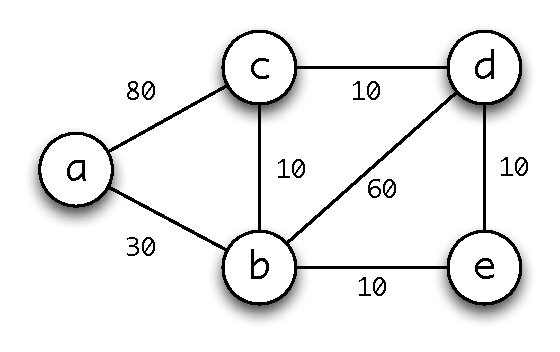
\epsfig{file=eps/flight-costs.eps,width=0.45\columnwidth}
\caption{Flight Map and Cost Between 5 Cities}
\label{fig:flight}
\end{figure}

\begin{figure}[tb]
\begin{lstlisting}[label=lst:tsell,caption=Ticket Seller's Agent. \texttt{[...]} denotes a list while \texttt{X[$i$]} is the $i$-th element of list \texttt{X}. \texttt{rand($m$)} returns a random integer between $0$ and $m$ (inclusive). \texttt{X.Y} denotes the concatenation of symbols so that \texttt{u.v} evaluates to \texttt{uv}.]
Ts = [[a,b,30],[a,c,80],[b,c,10],
      [b,d,60],[b,e,10],[c,d,10],[d,e,10]]
loop
  T = Ts[rand(6)]
  if rand(1) = 0
    |$\Out$|(ticket, T[0].T[1], T[2])
  else
    |$\Out$|(ticket, T[1].T[0], T[2])
|$\exit$|
\end{lstlisting}
\begin{lstlisting}[label=lst:tbuy,caption={Ticket Buyer's Agent. Both {\tt fly()} and {\tt try()} are defined using pattern matching on parameters. \texttt{[N:Ns]} denotes a list which has \texttt{N} as its head and \texttt{Ns} as its tail. Underscore (\texttt{\_}) matches anything in the context of pattern matching.}]
fly(X, X, Cash, V): arrived
fly(X, Y, Cash, V): Ns = unvisited_neighbors(X, V)
                    try(X, Ns, Y, Cash, V)

try(X, [N],    Y, Cash, V): buy(X, N, Y, Cash, V)
try(X, [N:Ns], Y, Cash, V): (buy(X, N, Y, Cash, V)
                            |$\oplus$|try(X, Ns, Y, Cash, V))
                            |$\cm$|

buy(X, N, Y, Cash, V):
  |$\In$|(ticket, X.N, |$\lambda x.x\le\texttt{Cash}$|) = (_, _, Cost)
  fly(N, Y, Cash - Cost, [N:V])

fly(a, e, 100, [a])
|$\exit$|
\end{lstlisting}
\vspace*{-5mm}
\end{figure}

\subsubsection*{Stock Trading (ST)}

In this example, we set up a mini stock market which follows the prices in the public exchange 
but is not openly available to the public. 
Traders can join the market at any time but their trades will not affect the public market.
Markets like this do exist in real life in the form of 
``Dark Pools''\cite{degryse2008shedding}  
which offers anonymous and private investors to
trade away from the public exachanges.

Our market starts with $N$ stocks, each has a fixed amount of shares dedicated for this market.
In general, each trader has a fixed amount of money in the beginning, 
and can buy (or sell) stocks from (or to) the market according to the public prices.
% Each trader also has a high watermark and a low watermark of cash.
% When the cash value is less than the low watermark (or greater than the high watermark), 
% the trader will keep selling (or buying) stocks in order to increase (or decrease) the cash value. 
% This strategy comes from real-world strategies where people want to control the risk.
% Different watermarks lead to different behaviors, and for this example, 
% the traders speculate to be either conservative or aggressive.
Listing \ref{lst:trader} shows the trader's agent program. 
Each trader trades several rounds until his cash value reaches the goal. 
For each round, the trader randomly picks a stock {\tt X}, buys it as much as possible, 
and waits for the price of {\tt X} to change. 
$\alpha$ is a value between 0 and 1 which indicates the profit/loss margin percentage. 
For example, if a trader buys {\tt X} at a price of {\tt P}, 
he sells it at a price of either higher than $(1+\alpha)\times{\tt P}$ (to profit)
or lower than $(1-\alpha)\times{\tt P}$ (to prevent further loss). 
Different $\alpha$ values lead to different trading behaviors, and for this example,
the traders speculate to be either 
conservative (smaller $\alpha$) or aggressive (larger $\alpha$).
Note that there is no atomicity guarantee between checking the price of a stock 
and actually buying it, which is also the behavior of a real market.
Also an intention to buy can be partially filled by the stock-serving agent
(see Listing \ref{lst:stock}).
The stock-serving agent also waits for price updating (i.e. {\tt (update, ...)})
from the public exchange in a realtime fashion. 

\begin{figure}[tb]
\begin{lstlisting}[label=lst:trader,caption={Trader's Agent. Numbers are irrelevant and just for illustration purposes.}]
Me     = unique_account_name
Stocks = [...]  // a list of stock names
Start  = 5000   // start with cash of $5000
Goal   = 5500   // the goal is to end up with $5500

trade(Cash, |$\alpha$|):
  X = Stocks[rand(N-1)]

  |$\Rd$|(price, X, _) = (_, _, P1)
  Q1 = |$\lfloor$|Cash / P1|$\rfloor$|
  |$\Out$|(buy, X, Q1, Me)
  |$\In$|(ack, Me, _, _) = (_, _, P2, Q2)
  C1 = Cash - P2 * Q2

  |$\Rd$|(price, X, |$\lambda x.x\ge(1+\alpha)\times{\tt P2}\lor x\le(1-\alpha)\times{\tt P2}$|)
  |$\Out$|(sell, X, Q2, Me)
  |$\In$|(ack, Me, _) = (_, _, P3)
  C2 = C1 + P3 * Q2

  if C2 < Goal
    trade(C2, |$\alpha$|)
  else
    |$\cm$|

trade(Start, 0.01) |$\oplus$| trade(Start, 0.05)
|$\exit$|
\end{lstlisting}
\begin{lstlisting}[label=lst:stock,caption=Stock-serving Agent. \texttt{P} is the current price of the stock while \texttt{Q} is the quantity of stocks available for sale.]
Me = unique_stock_name

serve(P, Q):
  case |$\In$|(_, Me, _, _)
    (update, _, NewPrc, _): |$\In$|(price, Me, _)
                            |$\Out$|(price, Me, NewPrc)
                            serve(NewPrc, Q)

    (buy, _, Q1, X): Q2 = min(Q1, Q)
                     |$\Out$|(ack, X, P, Q2)
                     serve(P, Q - Q2)
    
    (sell, _, Q2, X): |$\Out$|(ack, X, P)
                      serve(P, Q + Q2)

|$\Out$|(price, Me, Start_Price)
serve(Start_Price, Start_Quantity)
\end{lstlisting}
\vspace*{-6mm}
\end{figure}

\subsubsection*{Dining Philosophers (DP)}

% \begin{figure}[tb]
% \centering
% \epsfig{file=eps/dining.eps,width=0.3\columnwidth}
% \caption{Three Dining Philosophers Problem.
% $A,B,C$ are philosophers while $x,y,z$ are forks.}
% \label{fig:dining}
% \end{figure}

% \RY{can delete the figure. Listing 9 can be joined horizontally rather
% than vertically as now}

Consider the well-known ``Dining Philosophers Problem''
\cite{Dijkstra2002:Hierarchical} - there are three
philosophers $A$, $B$ and $C$, sitting around a dining table,
with three forks $x$, $y$ and $z$ between them.
This classic concurrency problem
shows that deadlock happens with certain sequences of acquiring the forks,
e.g., $A$ acquires $x$, $B$ acquires $y$ and then
$C$ acquires $z$. 
The classic solution to this problem is using a synchronization mechanism 
such as a counting semaphore, imposing a partial order on acquiring the forks, 
or requiring one philosopher to be asymmetric.
However, such kind of solution requires additional constraints to the problem. 
%
In this example, the speculation framework offers an alternative
solution which is purely based on the definition of the problem.
We extend the problem to $N$ dining philosophers 
sitting around a table with $N$ forks.
For simplicity, each philosopher has a unique index ranging from $0$ to $N-1$. 
Listing \ref{lst:dpinit} shows the initialization of data stores 
for dining philosophers.
Listing \ref{lst:dp} shows the agent program for dining philosophers.
\texttt{my\_index()} returns the index of the current philosopher.

\begin{figure}[tb]
\begin{lstlisting}[label=lst:dpinit,caption=Dining Philosophers (initialization)]
for I = 0 to N-1
  |$\Out$|(fork,I)
|$\exit$|
\end{lstlisting}
\begin{lstlisting}[label=lst:dp,caption={Dining Philosophers. \texttt{\%} denotes the modulo operation. {\tt ;} separates multiple statements in one line. $\Out$ is non-blocking in the tuple space data model, so we don't need choices for putting back forks.}]
L = my_index(); R = (L+1) % N
(|$\In$|(fork,L); |$\In$|(fork,R)) |$\oplus$| (|$\In$|(fork,R); |$\In$|(fork,L))
|$\cm$|
|$\Out$|(fork,L); |$\Out$|(fork,R)
|$\exit$|
\end{lstlisting}
\shrink
\shrink
\end{figure}

By using such kind of speculation, it can be guaranteed that 
there is always one world where nobody deadlocks. 
For example, assume $N=3$, the combination of the choices from three philosophers 
theoretically creates eight worlds as in Figure \ref{fig:diningrun} 
(though in practice some of the worlds may never be there due to pruning).

\begin{figure}
\centering\small
\Tree[.$\oplus_A$
    [.$\oplus_{B_1}$
        [.$\oplus_{C_1}$
            {$A\compact:-x$ \\ $\quad-y$ \\ $B\compact:-y$ \\ $\quad-z$ \\ $C\compact:-z$ \\ $\quad-x$ \\ $(w_1)$}
            {\bk$A\compact:-x$ \\ \bk$\quad-y$ \\ \bk$B\compact:-y$ \\ \bk$\quad-z$ \\ \bk$C\compact:-x$ \\ \bk$\quad-z$ \\ $(w_2)$}
        ][.$\oplus_{C_2}$
            {$A\compact:-x$ \\ $\quad-y$ \\ $B\compact:-z$ \\ $\quad-y$ \\ $C\compact:-z$ \\ $\quad-x$ \\ $(w_3)$}
            {\bk$A\compact:-x$ \\ \bk$\quad-y$ \\ \bk$B\compact:-z$ \\ \bk$\quad-y$ \\ \bk$C\compact:-x$ \\ \bk$\quad-z$ \\ $(w_4)$}
        ]
    ][.$\oplus_{C_3}$
        [.$\oplus_{B_2}$
            {$A\compact:-y$ \\ $\quad-x$ \\ $B\compact:-y$ \\ $\quad-z$ \\ $C\compact:-z$ \\ $\quad-x$ \\ $(w_5)$}
            {\bk$A\compact:-y$ \\ \bk$\quad-x$ \\ \bk$B\compact:-z$ \\ \bk$\quad-y$ \\ \bk$C\compact:-z$ \\ \bk$\quad-x$ \\ $(w_6)$}
        ][.$\oplus_{B_3}$
            {$A\compact:-y$ \\ $\quad-x$ \\ $B\compact:-y$ \\ $\quad-z$ \\ $C\compact:-x$ \\ $\quad-z$ \\ $(w_7)$}
            {\bk$A\compact:-y$ \\ \bk$\quad-x$ \\ \bk$B\compact:-z$ \\ \bk$\quad-y$ \\ \bk$C\compact:-x$ \\ \bk$\quad-z$ \\ $(w_8)$}
        ]
    ]
]
\caption{Three Dining Philosophers Problem (tree of choices). Minus sign ($-$) denotes taking the fork. Deadlock only happens in $w_1$ and $w_8$.}
\label{fig:diningrun}
\shrink
\end{figure}

There are many practical algorithms and applications (e.g., 2-phase locking)
that are special cases or extensions of the Dining Philosopher Problem (DPP). 
So we generalize DPP as follows.
\begin{definition}[Generalized Dining Philosopher Problem]
Given a set of resources $R$ which are available at the beginning, 
$n$ agents each interested in a subset of resources 
$R_i\subseteq R (1\le i\le n)$, and each agent is a two-phase process:
  \begin{enumerate}
    \item In the \emph{acquisition phase} the agent consumes every resource $r\in R_i$ in any order;
    \item In the \emph{release phase} the agent puts back every resource $r\in R_i$ in any order.
  \end{enumerate}
  $R_i$'s may overlap so the scheduler may produce a schedule which can cause deadlock 
among the agents.
\end{definition}

\begin{theorem} Generalized Dining Philosopher Problems do not deadlock 
using speculative nondeterminism.
\end{theorem}
\begin{proof}[Proof sketch]
% first show there is always a solution
First, we construct a combination of choices which will never deadlock. 
Fix an ordering of the elements in $R$, for example $r_1,r_2,\dots,r_m$ where $m=|R|$. 
For any agent $i$, it consumes $R_i$ in this fixed order. 
Then there will be races instead of deadlocks because there will not be the 
case that agent $i$ consumes $r_x$ and waits for $r_y$, and agent $j$ consumes
$r_y$ and waits for $r_x$ ($x<y$ and $y<x$ cannot be true at the same time). 
% then show the solution will not be pruned
Then it can be shown this combination will not be pruned by commits in an 
eventually blocking world due to the commit semantics described in rule \ref{rule:cm}. 
\end{proof}


\begin{figure}[ht!]
\centering
% TODO: use a tabular{cr} to format better
\flushright\fbox{Entrance transition: $T\|a\Longrightarrow T'$}
\[
  \tag{\sc Entrance1}\label{rule:entrance1}
  \langle A,D,S\rangle \| a \Longrightarrow \langle A+[a],D,S\rangle
\]
\[
  \tag{\sc Entrance2}\label{rule:entrance2}
  T_1\oplus_k T_2 \| a \Longrightarrow (T_1 \| a)\oplus_k (T_2 \| a)
\]
\flushright\fbox{Tree transition: $T\To T'$}
\[
  \tag{\sc Swap}\label{rule:swap}
  T_1\oplus_k T_2 \To T_2\oplus_k T_1
\]
\[
  \tag{\sc DataOp}\label{rule:dataop}
  \frac
  {A[k]=d.e:f \qquad D\vdash d \qquad \langle t,D'\rangle=\psi(d,D)}
  {\langle A,D,S\rangle \To \langle A[k\mapsto t.e:f], D', S\rangle}
\]
\[
  \tag{\sc Choice}\label{rule:choice}
  \frac
  {\begin{matrix}
    A[k]=(e_1\oplus e_2).e:f \\
    T_1=\langle A[k\mapsto e_1.e:f],D,S\rangle \\
    T_2=\langle A[k\mapsto e_2.e:f],D,S\rangle
   \end{matrix}}
  {\langle A,D,S\rangle \To T_1\oplus_k T_2}
\]
\[
  \tag{\sc Cm}\label{rule:cm}
  \frac
  {A[k]=\cm.e:f}
  {\langle A,D,S\rangle\oplus_k T \To \langle A[k\mapsto e:f],D,S\rangle}
\]
\[
  \tag{\sc Cu}\label{rule:cu}
  \frac
  {A[k]=\cu.e:f}
  {\langle A,D,S\rangle\oplus_k T \To T}
\]
\[
  \tag{\sc Exit1}\label{rule:exit1}
  \frac
  {A[k]=\exit.e :f \qquad s=\langle k,f(D)\rangle}
  {\langle A,D,S\rangle \To \langle A[k\mapsto\exiting],D,S\cup\{s\}\rangle}
\]
\[
  \tag{\sc Exit2}\label{rule:exit2}
  \frac
  {\begin{matrix}
    \forall w\in leaves(T): exiting(w,k) \land v = exitv(w,k)
   \end{matrix}}
  {T \To exit(T,k)}
\]
\[
  \tag{\sc Collapse}\label{rule:collapse}
  \frac
  {\begin{matrix}
    w \in leaves(T) \\
    \forall k: exiting(w,k) \lor exited(w,k)
   \end{matrix}}
  {T \To w}
\]
\flushright\fbox{Local computation transition: $e\computes e'$}
%\begin{align*}
\[
\begin{array}{llll}
  e &\computes op.e' \hspace*{5mm} &
  e &\computes \epsilon \\
  t.e &\computes e' &
  e_1.e_2 &\computes e_1'.e_2 \\
\end{array}
\]
%%  \epsilon.e &\computes e
%\end{align*}
\flushright\fbox{Helper functions}
\begin{gather*}
  \frac
  {T = T_1\oplus_k T_2}
  {leaves(T) = leaves(T_1)\uplus leaves(T_2)} \\
  leaves(w) = \lbb w\rbb \\
  \frac
  {w=\langle A,D,S\rangle \qquad \langle k,v\rangle\in S}
  {exitv(w,k) = v} \\
  \frac
  {w=\langle A,D,S\rangle}
  {exiting(w,k) = (A[k]=\exiting)} \\
  \frac
  {w=\langle A,D,S\rangle}
  {exited(w,k) = (A[k]=\exited)} \\
  \frac
  {T = T_1\oplus_i T_2}
  {exit(T,k) = exit(T_1,k)\oplus_i exit(T_2,k)} \\
  \frac
  {w=\langle A,D,S\rangle}
  {exit(w,k) = \langle A[k\mapsto\exited],D,S\rangle}
\end{gather*}
\caption{Semantics of the Speculation Language.
$[\dots]$ denotes a list,
$A[k]$ is the $k$-th element in list $A$, and
$A[k\mapsto x]$ denotes the updating of the $k$-th element to $x$.}
\label{fig:semantics}
\end{figure}

\subsection{Semantics}\label{sec:semantics}

The semantics of the speculation language is 
given in \figref{fig:semantics}. 

\paragraph*{Entrance}
New agents can dynamically enter the system at any time.
\ref{rule:entrance1} and \ref{rule:entrance2} the addition of
a new agent $a$ to the system (denoted $\|$). The Plus sign ($+$) 
denotes list concatenation. The whole tree is recursively traversed and $a$ is appended to the agent list in every world. 

\paragraph*{Choice Symmetry}
\ref{rule:swap} shows that the two branches of an interior node in the tree are treated equally.

\paragraph*{Data Operation}
An agent wants to execute operation $d$ on the data store $D$
(see \ref{rule:dataop}).
This transition first has to meet condition $D\vdash d$. 
The effect of $d$ on data store $D$ is defined by
the transition function $\psi$ in the data model and it only
affects the current world having store $D$
without affecting other worlds in the tree.
The result of $d$ is denoted is $t$ and provided to the remaining local 
computation $e$ as a parameter (denoted by the special syntax $t.e$). 
$t.e$ is not processed by the speculation framework, but 
activates the local computation $e$ and will eventually transform to another 
local computation $e'$ (i.e. $t.e\computes e'$). 

\paragraph*{Local Computation}
The local computation transition is simply a placeholder for
the semantics of the actual computation in the host language.
As that is orthogonal to our semantics, the details are left
unspecified. There is one special operation, $t.e$, which applies
the result of a data operation $t$ to some local computation $e$.
For example, it might be to store $t$ in a variable in the host language.
% \KZ{The following may need to be changed:\\
% We shall omit the details of the language in which 
% local computations are expressed and just assume that
% there exist a local computation transition $\computes$.
% From the perspective of the speculation framework, 
% the only thing that matters is the operation $op$ 
% produced by a local computation. 
% As shown in \figref{fig:semantics}, 
% a local computation $e$ transforms to $op.e'$ to 
% execute $op$ under the framework, or to $\epsilon$ to 
% finish execution. 
% After a data operation which reads something from the data store,
% a data item $t$ in the store is returned to the local computation $e$, 
% and further transforms to a new local computation $e'$, which is 
% $e$ parameterized by $t$. 
% $e_1.e_2$ denotes sequential execution of $e_1$ and $e_2$. 
% After $e_1$ transforms to $\epsilon$, $e_2$ starts execution 
% ($\epsilon.e\computes e$).
% }

\paragraph*{Choice and Commit}
Speculative nondeterminism provides for the creation and subsequent
pruning of choices. 
\ref{rule:choice} fires if an agent is reduced to a choice $(e_1\oplus e_2).e$, 
and it consumes the choice construct in the agent to split the current world into two
(i.e. $T_1$ and $T_2$). 
Section \ref{sec:commit} discusses further the ramifications of commit,
here, we start with first describing what the commit rules do.
When the $k$-th agent executes $\cm$ in a leaf world of the tree structure, 
as shown in rule \ref{rule:cm}, the other side of the choice (i.e. $T$) is pruned
only if the current choice node is $\oplus_k$. 
Similarly, $\cu$ is used where the agent wants to explicitly gives up the current choice branch,
so the current side of the choice is pruned, 
as shown in rule \ref{rule:cu}. 
$\cm$ and $\cu$ are symmetric and both of them are {\em commit} operators.
Commit of the $k$-th agent can only be executed in a world with $\oplus_k$ as its parent,
and it is blocking when the parent node is not $\oplus_k$.
%which makes the commit more localized and less aggressive. 
% This form of commit semantics is therefore known as {\em localized commit}.
%With this commit semantics, it only affects a small fraction of the whole tree. 
%Also it is possible to make pruning decisions locally, which makes it efficient. 

\paragraph*{Exit}
In general, a single agent will have many versions of itself executing
in all the multiple virtual worlds.
Thus, if it were simply to exit from all the worlds on the first
$\exit$ operation, this could lead to some form of data inconsistency.
We deal with this using the exit function $f$ specified by each agent which
allows an agent-specific consistency condition to be used.
Note that different agents may be interested in different aspects of the data store. 
When an agent exits, all the worlds should look the same from the perspective of that agent. 
However, another agent may not consider the worlds to be the 
same since it can have a different exit function. 
This also means that an agent properly exiting is only achieved when
the consistency requirement is obtained.

Rule \ref{rule:exit1} and \ref{rule:exit2} shows the exit semantics. 
\ref{rule:exit1} shows the case when an {\em instance} 
of the $k$-th agent reaches $\exit$ in a world. 
In this case, the exit function $f$ is applied to the current data store $D$ and a {\em snapshot} 
is created and added to $S$. 
 
The exit function $f$ takes a data store as input, and returns an integer as the evaluated result. 
The data store is just the one associated with the current world. 
According to the data store, the exit function is expected to produce an integer 
which can be a 0/1 indicator, a heuristic value, or an encoding of more complicated mathematical objects. 
For example, in the simplest case, $f(d)\equiv 1$ allows the agent to exit without any condition 
as long as it completes execution of all the operations in the program. 
The ability to return an integer provides more flexibility and enables 
complex exiting logic to be embedded in this exit function.

While taking a snapshot, 
the agent in that world switches to a special state $\exiting$.
\ref{rule:exit2} checks all the worlds in the tree. Only if (i) the $k$-th agent has 
switched to $\exiting$ state in all the worlds, and (ii) the exit value $v$ of the $k$-th agent 
is {\em identical} across all the worlds, 
then the $k$-th agent can exit from the worlds at the same time. 
For \ref{rule:exit2}, the exit value $v$, which can be thought of as the return value from
the speculative computation, will be eventually provided to 
a local computation $\tilde e$
which is completely outside the system of virtual worlds, 
and has no more speculation and data store operations. 
The idea of this type of consistent exit across all worlds is analogous
algebraic factorization, i.e.
$ab + ac = a(b+c)$.

\paragraph*{Collapse}
Note that commit is optional in an agent program, so the agents can 
let the tree expand without pruning, and finally leave the tree 
without reducing to one world. 
Therefore some agents may never exit due to the inconsistency of some worlds, 
even if all the agents have finished execution.
\ref{rule:collapse} handles this case 
to let these agents exit as well as to reclaim system resources. 
The system could employ a global collapse rule to pick any world where 
all agents have completed execution and reduce the tree to one world.
For \ref{rule:collapse}, the exit value for every agent $k$ is also returned in this way.
$\tilde e$ can make use of the exit value to extract what the agent concerns. 
%\KZ{Need to say exit is implicit if it's not added to the program?}

\paragraph*{Helper Functions}
We also define a set of helper functions to simplify the semantics. 
\begin{description}
\item[$leaves(T)$] returns a multi-set of the leaf worlds in tree $T$. 
\item[$exitv(w,k)$] retrieves the exit value, i.e. the evaluation result of the exit function, of the $k$-th agent in world $w$.
\item[$exiting(w,k)$] is a predicate indicating whether the $k$-th agent in world $w$ is in the special state of $\exiting$.
\item[$exited(w,k)$] is a predicate indicating whether the $k$-th agent in world $w$ is in the special state of $\exited$.
\item[$exit(T,k)$] switches the $k$-th agent in all the worlds in $T$ to the special state of $\exited$.
\end{description}

\subsection{More on Commit}\label{sec:commit}
Commit is a special and important operation in speculative nondeterminism because:
(i) it gives the agent the power to specify preferences among different choices,
e.g., in Listing \ref{lst:intro-commit-sleep}; 
(ii) it prunes some of the virtual worlds to make it easier for agents to exit
because the fewer remaining worlds means easier consistency checks,
and thus it improves the responsiveness and overall throughput of the system;
(iii) by pruning worlds, it also reclaims precious system resources such as
memory and CPU cycles, which is critical to the viability of the multi-world 
speculation , even though the naive combinatorial problem space is exponential and
prohibitive.

However, it is also important to understand that whenever commit is used and
pruning is done, potential solutions can be pruned away, and deadlock or blocking
may arise as a result. So from the system point of view, we design a commit
semantics that is {\em localized} and less aggressive because the scope of the pruning
is restricted to be of height 1 only and affects only a small fraction of
the whole tree (see Rule \ref{rule:cm}). This commit semantics is also
more efficient because pruning decisions are made locally. There are of course
other possible commit semantics \cite{JaffarYZ07} which are more eager in pruning. 
For example, one type of commit requires agent $T$ to commit in all left or right
subtree rooted at $\oplus_T$. These are either too aggressive and lose 
too many solutions or require coordination
among various worlds which is more costly to execute in practice.

From the programmer's point of view, she should use commit with care, knowing that
without commit, the multi-world space grows very quickly and the program probably
cannot scale, but with commit, the program could potentially lose valuable solution.
It makes more sense to put commit later rather than early in the choice. 
If one must put a commit in the middle of a sequence of operations like
$op_1.op_2.\cm.op_3.op_4$, she should ensure that the remaining operations
after $\cm$, i.e., $op_3$ and $op_4$, are not likely to block, 
e.g., when they are local computations.

%The commit semantics described in Section \ref{sec:semantics} 
%is called {\em localized commit} as it restricts
%the scope of pruning to be of height 1 only.  
%%$\cm$ by agent $X$ cannot
%%prune until the direct parent of the committed world is $\oplus_X$.
%%$\cu$ kills the current world immediately without coordination with other worlds.
%Besides localized commit, there is a number of other possible commit
%semantics \cite{JaffarYZ07}.
%They differ in their eagerness to prune the worlds.
%They are ordered roughly from the most eager to the most conservative:
%{\em absolutely eager commit}, {\em eager commit}, {\em coordinated commit}, 
%{\em late commit} and {\em no commit}. 
%



\section{Framework Overview}
\label{sec:system}

\begin{figure}[th]
\centering
\includegraphics[width=1.0\columnwidth]{picture/framework.eps}
\caption{ICQ Workflow. Dotted arrows indicate the visualization of 
the distributions.}
\label{fig:framework}
\end{figure}

The overview of ICQ framework is illustrated in in~\figref{fig:framework}. 
With ICQ, we can detect whether a model is 
sensitive to a particular linguistic feature during inference with a 
stress test.
Next, we present some of the linguistic features used in this framework,
and then explain how ICQ works in more details.
%\KZ{The following is not right, things are not mentioned in the fig at all: 
%ICQ can be broken down into the following phases: feature definition, 
%dataset filtering, and model evaluation. With ICQ, we 
%discover whether the data have spurious cues, and whether a model is 
%sensitive to a particular linguistic feature during inference.
%}
%WeWe evaluate the information leak in the datasets by statistical cues only. 
%First, we formulate  a number of NL reasoning tasks in a general form. 
%Then based on the cues associated with each label, 
%we design a number of metrics to measure the correlation between words
%and labels. Such correlation scores are called ``cue scores'' because they are 
%indicative of potential cue patterns. Afterwards, we aggregate the scores using a number of simple statistical
%models to make the predictions. Finally, we show how to split a dataset into
%the easy and hard parts using the above fast predictions.

\subsection{Linguistic Features}
\label{sec:extract}

In this work, we have considered the following list of linguistic features: 
Word, 
Typos, NER (appropriately understanding named entities), 
Tense (understanding temporal order of events), Negation, 
Sentiment, and Overlap (overlapping words between premise and hypothesis). 
This list is by no means exhaustive, but just a starting point for users, 
who can come up with additional features that are specific 
to their task or domain. We use $F$ to denote the feature set.

\subsubsection{Word} For a dataset $X$, 
we collect a set of all words that exist in $X$. We only consider unigram words in datasets.
%These 
%words can be word or cross-word that consists of a pair of
%unigrams, one from the premise and other from the hypothesis.
%the token pair between $p$ and $h$.
%We use conditional probability as feature metric for a word measures the 
%disparity of the word's appearance under 
 %a specific label.
%The cross-unigrams, such as  ``swimmer-sea'' in~\exref{exp:snli}, 
%represent the 
%relational unigrams in a dataset. 
%The ``swimmer-sea'' cross-unigram can be identified as a cue if it always appear in the instances with 
%one label, like entailment.

%Let $w$ be a word in $\mathcal{N}$, we compute a scalar statistic metric 
%called {\em cue score}, $f^l$, for a label $l$. 
%We use conditional probability(CP)
%as the feature score to measure the correlation between words and labels: 
%\begin{equation}
%    cp^{(w,l)} = \frac{\#(w, l)}{\#(w)}
%\end{equation}

%We rank the words by feature score to $N^{'}$ and 
%only treat top $k$ words as features:

%\begin{equation}
%    F_{W_i} = {w}_{i} , i \in 1...k \wedge w_{i} \in N^{'}.
%\end{equation} 

%We further define accuracy deviation score ($\mathcal{D}$)
%\begin{equation}
%    \mathcal{D} = {Acc} - {Majority},
%\end{equation}
%where $Acc$ is the prediction accuracy of a simple logistic regression
%model trained on the CP feature of all words or of a hypothesis-only
%model, and $Majority$ is the accuracy of vote by majority.
%As \figref{fig:d_figure} shows, accuracy of the linear model using 
%the CP features is very similar to the more complex hypothesis-only models 
%(Pearson score of 97.17\% for fastText and 97.34\% for Bert), 
%which indicates CP is a good choice of word feature.

%\begin{figure}[th]
%\centering
%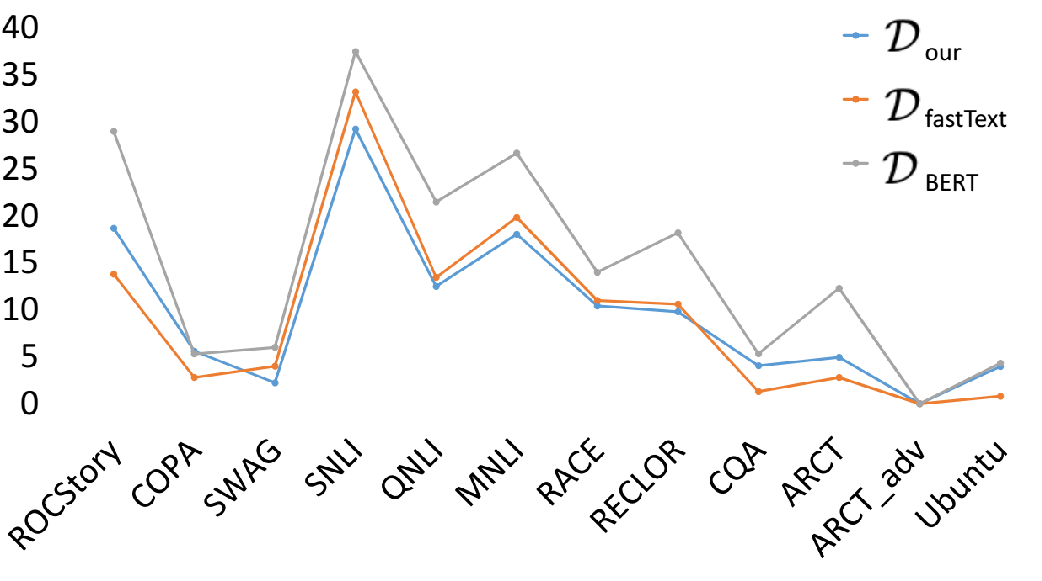
\includegraphics[width=0.7\columnwidth]{picture/d_figure.pdf}
%\caption{Deviation scores for three prediction models on all 12 datasets. 
%``Our'' means our logistic regression model.}
%\label{fig:d_figure}
%\end{figure}

%of $w$ with respect to label $l$ as
%%\KZ{Consider changing $\mathcal{F}$ to $\mathcal{B}$ to avoid confusion with $f$?}
%
%\begin{equation}
%    f_{\mathcal{F}}^{l} = f_{\mathcal{F}}(w, l),    
%\end{equation}
%%We call $f_{\mathcal{F}}^{(k,l)}$ \textit{cue metric}, 
%where $f_{\mathcal{F}}^{l}$ is a function which measures how much spurious information can be conveyed by token $w_k$ for a particular label $l$. 
%$\mathcal{F}$ is a set of cue metrics that we used for computing the \textit{cue score}. 

\subsubsection{Sentiment}

We assign sentiment features as 
positive, negative, or neutral to each hypothesis $h$: 
$sentiment(h) = \sgn(\mbox{num of positive words} - \mbox{num of negative words})$.
%in the hypothesis.
The sentiment polarity of a word
is determined by a look-up from pre-trained
sentiment lexica\footnote{NLTK: \url{https://www.nltk.org}}. 

\subsubsection{Tense}

Considering that the temporal order of events can be also 
important information for inference tasks, we include 
\textit{past}, \textit{present}, \textit{future} as Tense features. 
The tense is determined by verb tags after POS tagging.

\subsubsection{Negation}

Much work has observed that strongly negative words (``no'', ``not'') 
cause the model to predict contradiction for
neutral or entailed statements. Thus we think negation feature can be a factor which affects models in decision-making. 
Negation is decided by dependency parsing~\footnote{Scipy: \url{https://www.scipy.org}}.

\subsubsection{Overlap}
In many cases, substantial word-overlap between the premise and the
hypothesis sentences causes wrong entailment prediction, 
even if they are unrelated. 
%Very little word overlap causes a prediction
%of neutral instead of entailment. 
Thus we wonder 
whether overlap feature really influences models. 
We filter stop words, for example ``a'' and ``the'', before investigating overlap feature. 


\subsubsection{NER}
%\KZ{Rephrase this: The failure for the NER tests in CheckList
%indicates that these models are relying on shortcuts.}
Checklist constructs some stress tests for some NER features. The performance 
of models dropped heavily which indicates that these models are not robust and may 
take advantage of shortcuts.
For example, some name like ``Tom'' mostly appears with label ``contradiction'' 
may influence the decision of models.
%For example anchoring on named entities too strongly
%instead of understanding the reasoning behavior. 
We take NER features, like \textit{location}, \textit{person}, \textit{orgnization}, in our feature test.

\subsubsection{Typos}
The premise or the hypothesis is ill-formed because of spelling errors. 
Typo feature may also be learned by models as off-site information. 
We use a pretrained spelling model~\footnote{\url{https://github.com/barrust/pyspellchecker}} 
to detect the typos in a sentence. 

%We only pay attention to the features which have enough test data for model evaluation.
%In addition, we can analysis the credibility of test data through 
%the Kullback-Leibler (KL) Divergence. If a train dataset distribution is unbalance, 
%a similar distribution between train and T
%test can lead to insufficient test which test the cues mostly with a certain label. 

%\subsection{Data Set Filter}
%\label{sec:generate}
%Given the features $F$, 

%distribution and red distribution represent  the training and test data 
%distribution on the predication values respectively.  
%We use mean square error (MSE) to measure the balance 
%of a feature in a dataset. If the filtered training data distribution is 
%unbalanced on a feature, this feature can be seen as bias.  
%If this bias also exists in test data, indicating 
%a similar distribution exists in the test data, 
%this feature is considered a cue. 

%We show the distribution of some filtered SNLI datasets 
%in~\figref{fig:dataset_result}. 
%We can see that Word feature ``speaking'' mostly correlates with 
%label ``entailment''. So ``speaking'' is a bias. 
%The similar shape between the training and test data distribution indicates 
%this bias is a cue. Low Jensen-Shannon Divergence (JSD) score between the two
%distributions re-affirms our conclusion. 
%Compared with ``speaking'', Word feature ``pushing'' has lower MSE 
%score, but is still much higher than average distribution.  
%Thus ``pushing'' is also a bias. However we can observe that there is little similarity between 
%the train and test distribution. Therefore ``pushing'' is not a cue.
%With filtering and visualizing, we can analysis the biases 
%and cues in datasets. 
%Biases can influence models and cues make the evaluation unauthentic. 

%\begin{figure}[th]
%\centering
%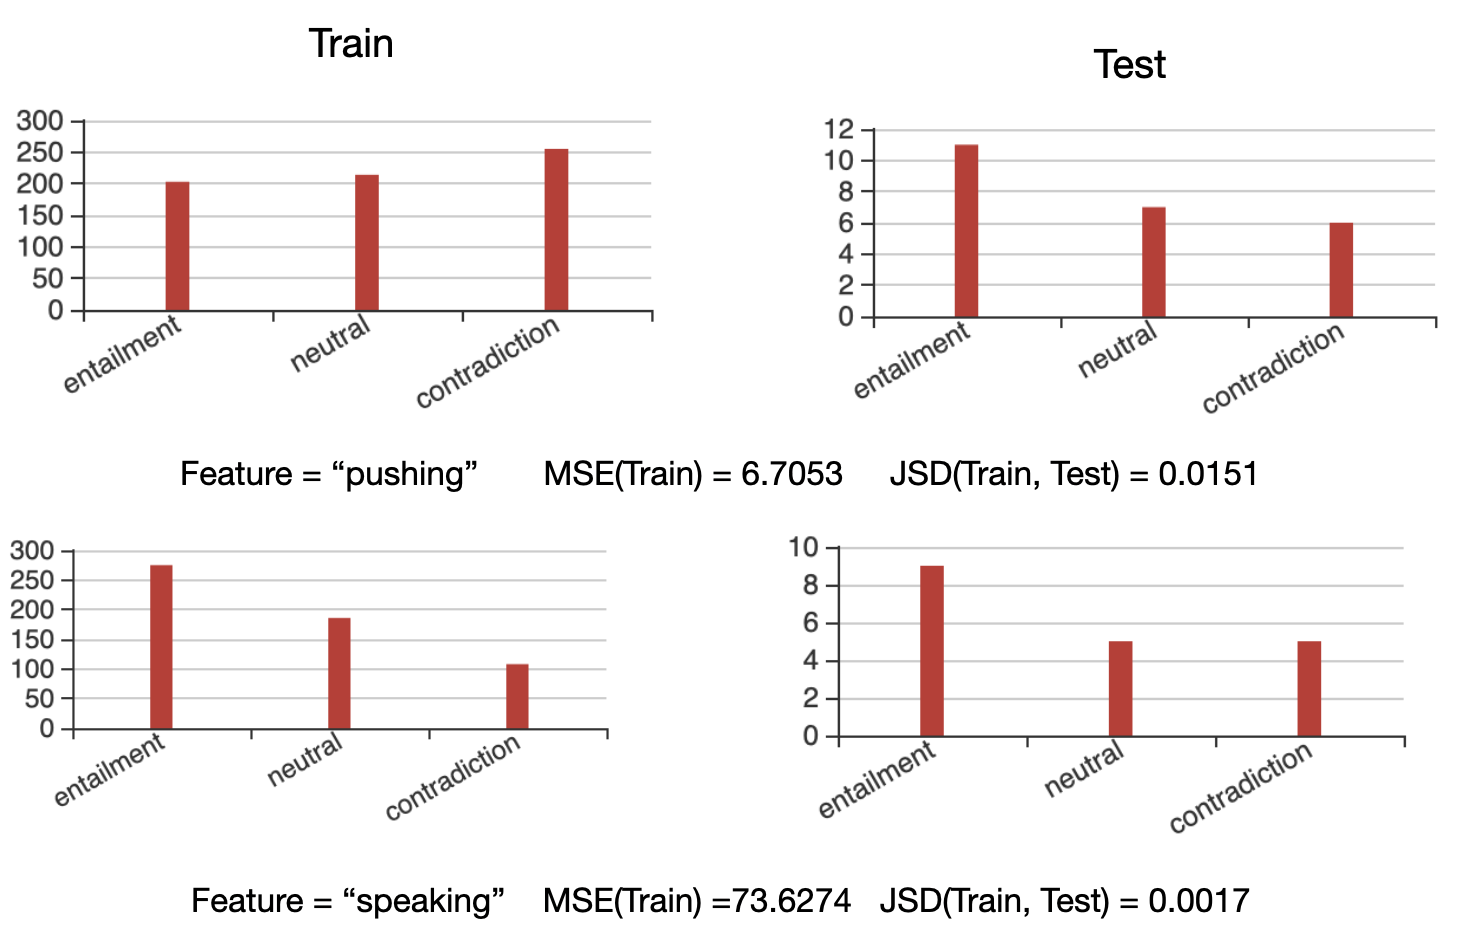
\includegraphics[width=1.0\columnwidth]{picture/dataset_result.jpg}
%\caption{Two examples of dataset distribution on features.}
%\label{fig:dataset_result}
%\end{figure}

\subsection{Model Evaluation}
\label{sec:model}

%We filter cases with specific features $F$ from the training and test data. 
For a specific feature, we filter the examples related to this feature from training and test dataset in~\figref{fig:framework}. 
For example, if we concern about ``Negation'' feature, we will extract all samples which contain negation tags on its parse tree. We can get feature distribution of filtered training data based on each label which is used as a reference for the model prediction distribution. The filtered test data is used to generate stress test that will be introduced in the following. 
In this filtering process, we don't retrain the model or change 
the parameters of models.

%Similar to discovering biases and cues, 
For investigating the bias of models, we can probe models by  
comparing the distribution of the model prediction results and 
the training data. We use JSD here to represent the deviation. 
The smaller the value of JSD, the more the model is affected 
by the distribution of training data.
%but don't provide new method for data augmentation. 
%We require a more fair dataset to test if a model is sensitive to a feature. 
The filtered test dataset of a feature in \figref{fig:framework} (red) is unbalanced among 
labels. The number of cases for each label can be denoted as $c_{ent}, c_{neu}, c_{con}$~(in 
SNLI task). If any of these number is smaller than a threshold $\sigma$, 
we won't consider this feature as a cue at all, because
 this feature is not well supported by enough data. 
%If the smallest number of samples among different labels is lower than 
%a threshold $\sigma$, we won't consider to test this feature. Because
% this feature is not well supported by enough data. 
%The smallest number can be denoted as $c_{min}=min(c_{ent}, c_{neu}, c_{con})$.
The maximum number can be denoted as $c_{max}=max(c_{ent}, c_{neu}, c_{con})$.
To make the result more intuitive and fair, 
we flatten the distribution by repeating $c_{max} - c_{l}$ cases from the filtered cases with label $l$ 
resulting in the orange ``stress test'' 
in \figref{fig:framework}. 
Then we test the model on this stress test. 
The similarity between prediction result (green) and 
training data distribution (blue) on a feature indicates how the model 
is influenced by the appearance of this feature in training data. 
For example, in \figref{fig:model_result}, we use 
ESIM~\cite{chen2016enhanced} model on SNLI. 
We can find that the model is affected by some bias features. 
Given ``pushing'', it still prefers to choose \textit{contradiction}. 
Further, it prefers to choose \textit{entailment} or \textit{neutral} with ``speaking''.  
JSD score for these two examples are also very low. 
%With comparison, we can find that models are sensitive to some bias features. 

%It is insufficient for testing if the filtered test data size is quite small or samples on 
%some label is rare which bellow a threshold $\sigma$. 
%Thought we can't generate cases for feature, we can point out what kind of 
%test samples should be augmented. 

\begin{figure}[th]
\centering
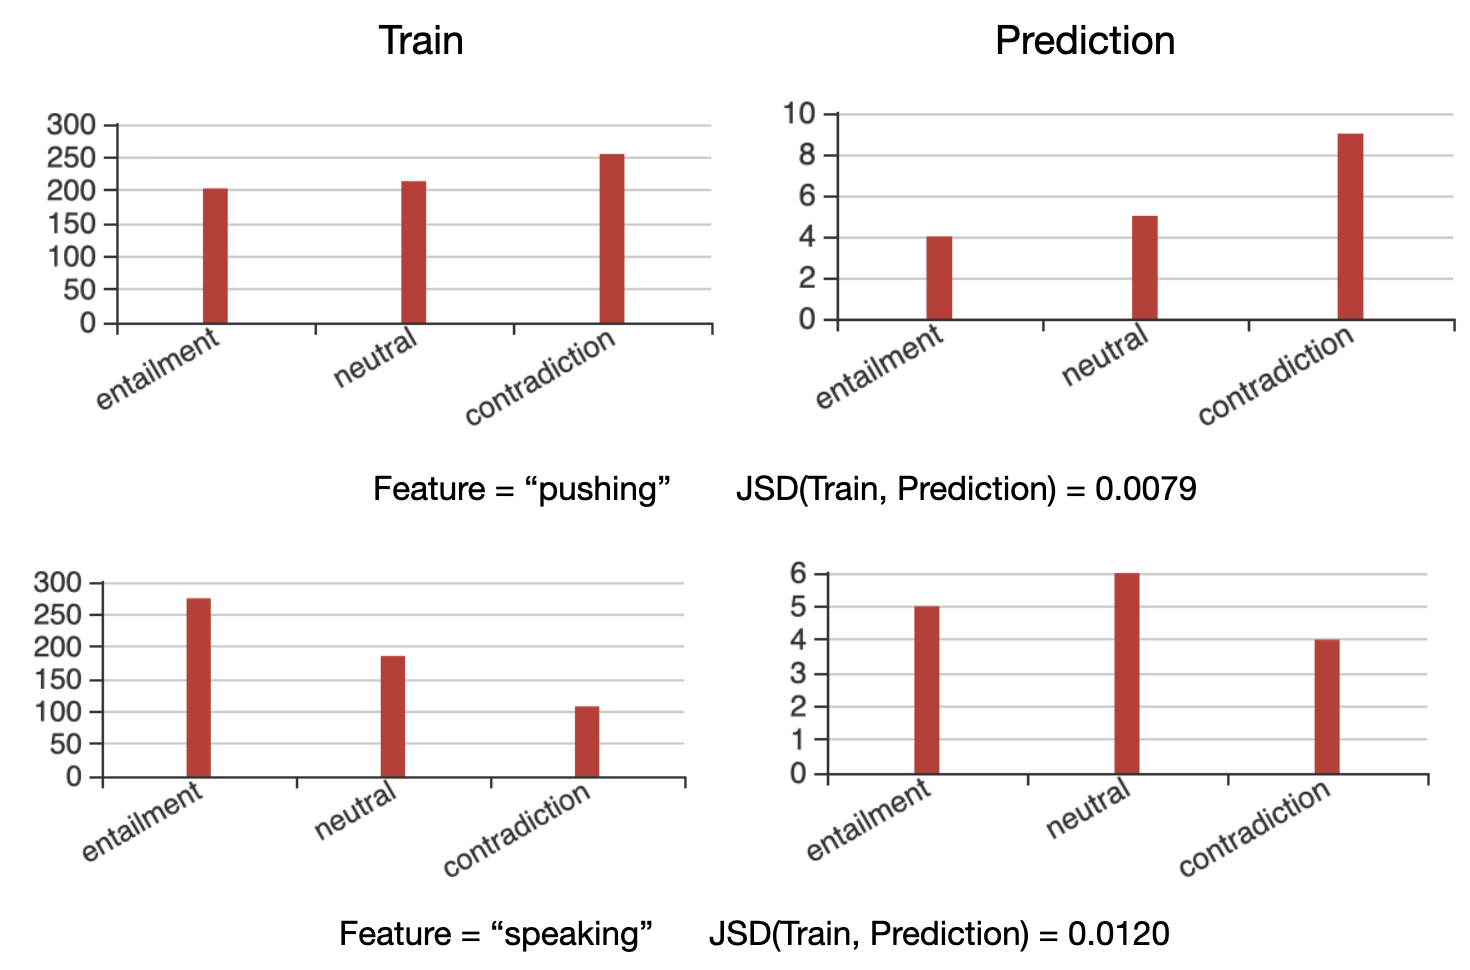
\includegraphics[width=1.0\columnwidth]{picture/model_result.jpg}
\caption{Two examples of model prediction result distribution on features.}
\label{fig:model_result}
\end{figure}


%The similarity is 
%calculated by Kullback-Leibler (KL) Divergence.

\section{Experiment Evaluation}
\label{sec:experiment}
In this section, we first give some statistics of our corpus and evaluate the quality and quantity of the learned rules. Then, we compare with other causal knowledge bases. Next, we analyze and discuss some main sub-modules in the rule learning framework. Finally, a practical application of futures price prediction and demonstration are introduced. Our experiments are implemented in Python and SWI-Prolog\footnote{ \url{ http://www.swi-prolog.org/}}.
% and run on a computer with Intel Xeon 32 CPU(2.60GHz) and 173GB memory.
	
\subsection{Dataset}
We crawled the text dataset from Chinese financial news website \footnote{\url{ http://finance.sina.com.cn}}. The news data containing 4,991,000 articles, from 2000/7/20 to 2017/12/31, is used to rule learning.
%	, which are split into \textbf{111,330,205} sentences. The number of unique sentences is \textbf{75,572,053}, covering  \textbf{67.88\%} of the total sentences. 
The number of sentences with causal cue words is 7,147,141, accounting for 9.46\% of the total number of de-duplicated sentences (75,572,053. The repetition rate of sentences is about 32\%).
It shows that about  \textbf{14.2\%} (9.64\%/(1-32\%)) sentences explicitly express causality in online financial news sentences.
The news data containing 270,562 articles, from 2018/1/1 to 2018/11/2, is used to evaluate our framework. We set $\alpha$ to 0.5 to achieve an equal balance between generalization and specialization in rule induction. 
We set $\gamma$ to 0.3 to control the Prolog engine to reason around two steps, since more than two steps lead to obviously unreasonable results.

%	\begin{table}[]
%		\caption{Dataset Information}
%		\begin{center}
%		\begin{tabular}{|l|l|l|}
%			\hline
%			Dataset       & Train & Test \\ \hline
%			Time Interval &       &      \\ \hline
%			Number        &       &      \\ \hline
%		\end{tabular}
%	\end{center}
%	\end{table}

\subsection{Rule Evaluation}
We evaluate these rules both quantitatively and qualitatively.
\paragraph{Quantitative Evaluation}
The number of the final rules we learned is \textbf{50000}. We divide the rule quality into three levels: good, fair and bad. According to the ranking of rule confidence, we randomly select 200 rules from the top 10000 rules and manually divide them into three levels. The `good', `fair', and `bad' levels of them account for \textbf{32.5\%}, \textbf{39.0\%} and \textbf{28.5\%}, respectively.
%	\begin{table}[]
%		\centering
%		\begin{tabular}{|l|l|l|} \hline
%		 good & fair &bad \\ \hline
%			65/200(32.5\%)& 78/200(39.0\%) & 57/200(28.5\%) \\ \hline
%		\end{tabular}
%		\caption{Rule Quality}
%		\label{tab:rule_quality}
%	\end{table}

\paragraph{Qualitative Evaluation}
%\begin{align*}
%%	good
%%	{"c": ["过剩_1", "X_燃料", "产量", "", ""], "e": ["下降_1", "X_自然资源", "价格", "", ""], "relation": [["c_sc", "e_sc", "madeof"]], "ctx": {"senids": [1975666], "pattern_ids": [8]}, "ruleid": 5131, "confidence": 0.5657637042081998}
%&\text{1 (X, '产量/yield', '过剩/surplus', '', ''):-(Y, '价格/price', '下降/fall',} \nonumber\\
%&\text{'',''), IsA(X, '燃料/fuel'), IsA(Y, '自然资源/natural resource'),} \nonumber\\
%&\text{madeof(X, Y)} \\
%%{"c": ["结束_1", "X_国家", "罢工", "", ""], "e": ["下降_1", "X_金属", "价格", "", ""], "relation": [["e_sc", "c_sc", "atlocation"]], "ctx": {"senids": [341012], "pattern_ids": [6]}, "ruleid": 11607, "confidence": 0.5824045924950126}
%&\text{2 (X, '罢工/strike', '结束/stop', '', ''):-(Y, '价格/price', '下降/fall', }\nonumber\\
%&\text{'',''), IsA(X, '国家/nation'), IsA(Y, '金属/metal')}\nonumber\\
%&\text{, atlocation(Y, X)}	 \\
%%{"c": ["下降_1", "X_作物", "价格", "", ""], "e": ["减少_1", "", "", "X_作物", "面积"], "relation": [["c_sc", "e_oc", "=="]], "ctx": {"senids": [961411], "pattern_ids": [8]}, "ruleid": 978, "confidence": 0.5876590112986869}
%&\text{3 (X, '价格/price', '下降/fall', '', ''):-(X, '面积/area', '减少/fall', }\nonumber\\
%&\text{'',''), IsA(X, '作物/crop')} \\
%%fair
%%2{"c": ["下降_1", "X_国家", "储蓄率", "", ""], "e": ["下降_1", "X_国家", "增长率", "", ""], "relation": [["c_sc", "e_sc", "=="]], "ctx": {"senids": [1640122], "pattern_ids": [5]}, "ruleid": 213, "confidence": 0.7185889172176277}
%&\text{4 (X, '储蓄率/saving rate', '下降/fall', '', ''):-(X, '增长率/growth rate', }\nonumber\\
%&\text{'下降/fall','',''), IsA(X, '国家/nation')} \\
%%2{"c": ["下降_1", "", "X_产品", "", ""], "e": ["适合_1", "", "X_作物", "", ""], "relation": [["c_s", "e_s", "madeof"]], "ctx": {"senids": [1791763], "pattern_ids": [6]}, "ruleid": 19783, "confidence": 0.5634539402859007}
%&\text{5 ('', X, '下降/fall', '', ''):-('', Y, '适合/fit', '', ''), IsA(X, }\nonumber\\
%&\text{'产品/product'), IsA(Y, '作物/crop'), madeof(X, Y)}   \\
%%bad
%%1{"c": ["减少_1", "", "X_国家", "X_自然资源", "依赖性"], "e": ["增加_1", "", "", "X_燃料", "销量"], "relation": [["e_oc", "c_oc", "madeof"]], "ctx": {"senids": [1707156], "pattern_ids": [8]}, "ruleid": 4468, "confidence": 0.5717182258485046}
%%另一方面,由于日本、韩国和中国减少对中东地区进口原油的依赖性,道达尔公司希望增加对这三个国家的液化天然气销量。
%&\text{6 ('', X, '减少/fall', Y, '依赖性/dependence'):-('', '', '增加/increase',}\nonumber\\
%&\text{ Z,'销量/sales'), IsA(X, '国家/nation'), IsA(Y, '自然资源/natural-} \nonumber\\
%&\text{resource'), IsA(Z, '燃料/fuel'), madeof(Z,Y)}	
%\end{align*}
Figure \ref{fig:rules_case} shows some typical rules: 1,2,3 are good, 4,5 are fair, and 6 is bad.
The main problems of these rules include:
The extracted events are not incomplete, which makes the rules less informative, such as rule 4 and 5.
The causality between cause event and effect event is not very strong, which should be attributed to the design of causal patterns and the process of rule induction, such as 4 and 6.
Some other problems also exist, such as verb disambiguation when normalizing predicates, noun disambiguation when generalizing rule instances.
%	\begin{figure}[htbp]
%	\begin{center}
%		
\includegraphics[width=0.95\columnwidth]{figures/reasonable_rule_case}
%	\end{center}
%	\caption{Examples of reasonable Rules.}
%	\label{fig:reasonable_rule_case}
%	\end{figure}
\begin{figure}[htbp]
	\centering
	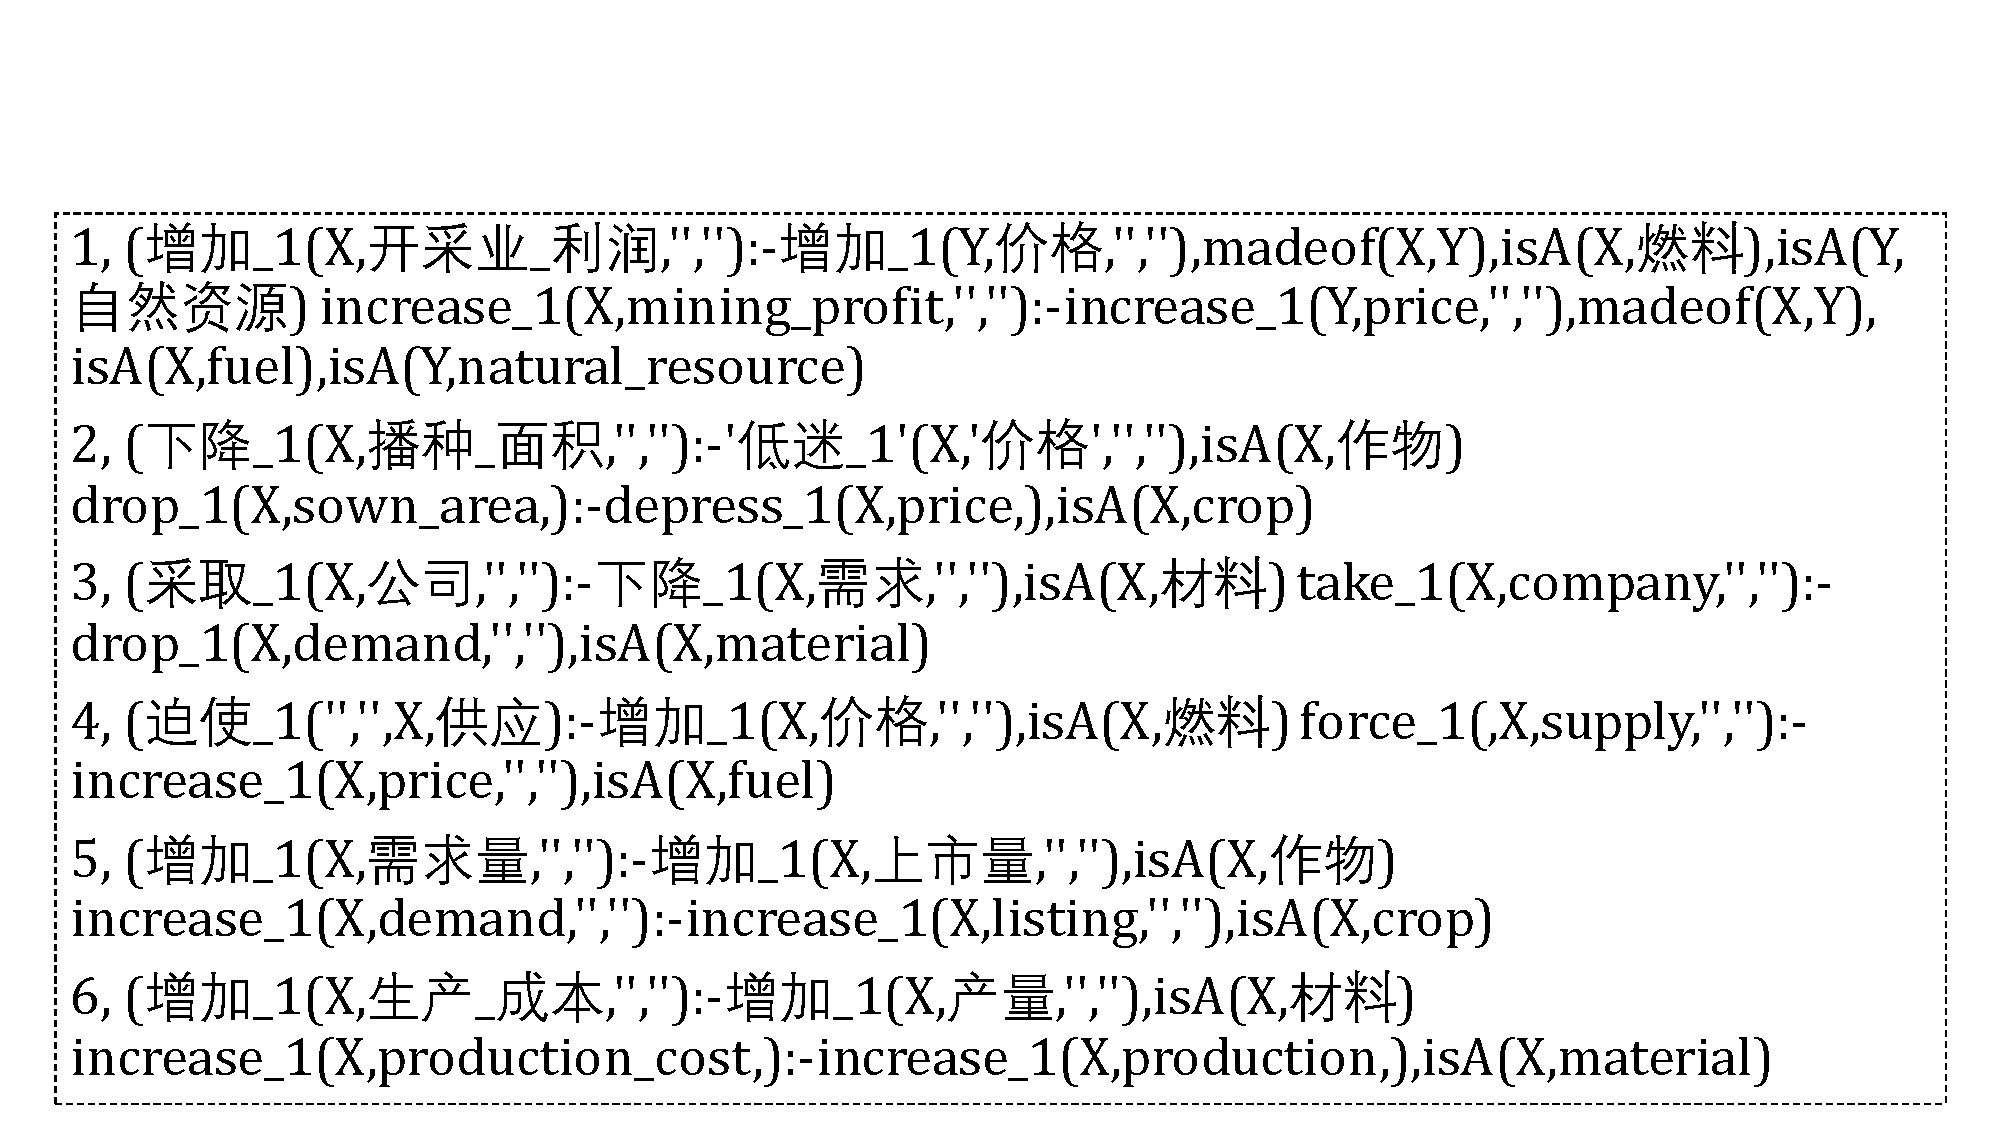
\includegraphics[width=0.95\columnwidth]{figures/rules_case}
	\caption{Examples of Typical Rules}
	\label{fig:rules_case}
\end{figure}
\paragraph{Event Graph}
With these rules, we deduce many rule instances with Prolog and pick out a tiny subgraph about rise and fall events, in Figure\ref{fig:rule_instantiation_graph}, to show the power of the rules. 
	
\begin{figure}[htbp]
\begin{center}
	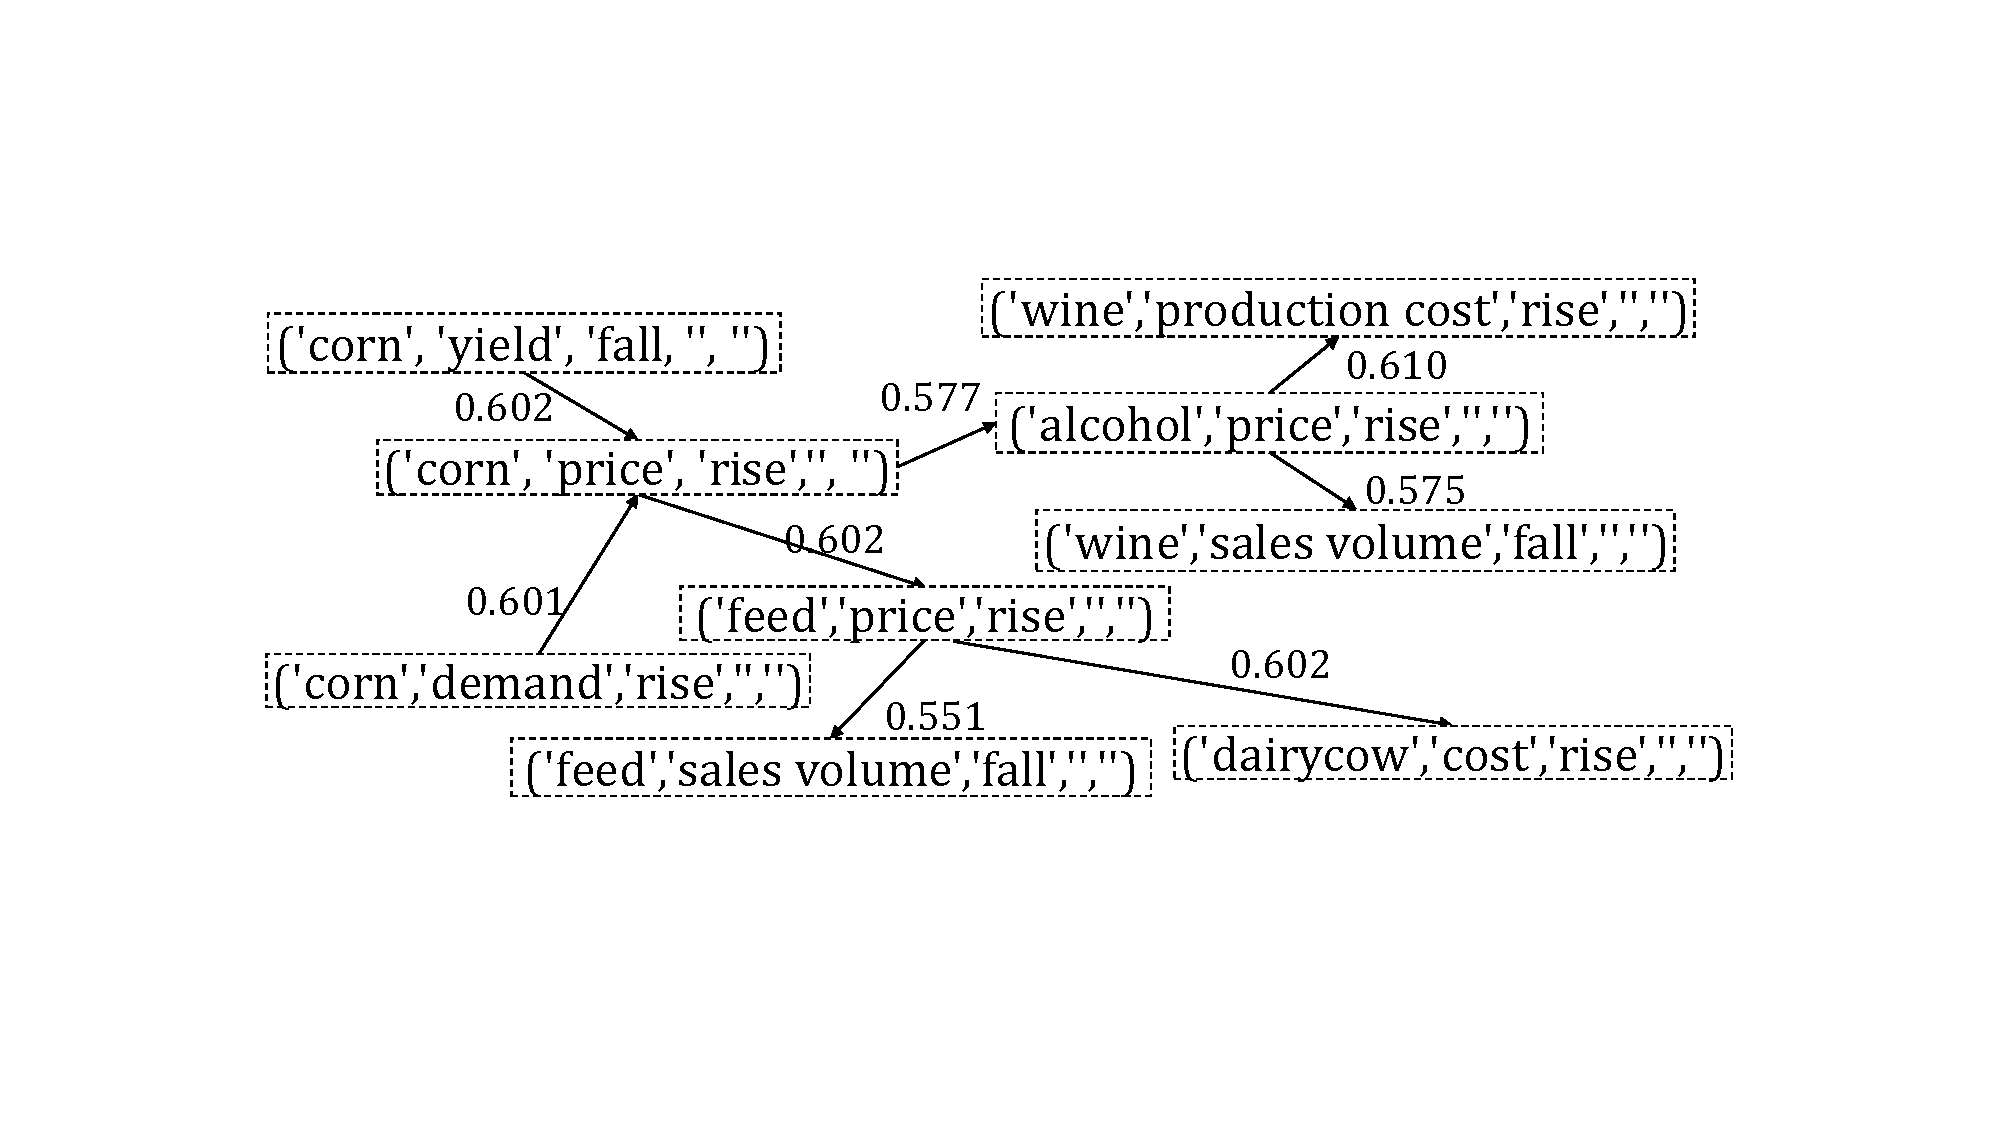
\includegraphics[width=0.9\columnwidth]{figures/instantiation_graph}
\end{center}
\caption{Rule Deduction. As space is limited, we only show the English version and omit the rules used in the reasoning process.}
\label{fig:rule_instantiation_graph}
\end{figure}

\subsection{Comparison with existing Knowledge Bases}
We compare our rules with causal part of other knowledge bases in various aspects in Table \ref{tab:comparison_rule_with_kbs}. We can see our causal knowledge representation is more expressive and informative, and the automatic knowledge acquisition is very convenient.
\begin{table*}[htbp]
\centering
%\begin{tabularx}{\columnwidth}{|c|c|c|c|}\hline
	\begin{tabular}{|c|c|c|c|c|c|c|c|}\hline
	\textbf{Name}&\textbf{Number}&\textbf{Domain}&\textbf{Unit}&\textbf{Data Structure}&\textbf{Information}&\textbf{Source}&\textbf{Precision}\\ \hline
	CausalNet&\textbf{62,675,002}&\textbf{Open}&word&(-)&rich&\textbf{automatic}&-\\
	\multicolumn{8}{|c|}{(`drink',`accident',36)}\\\hline
	ConceptNet &89,416&\textbf{Open}&short text&unstructured&rich&crowdsourcing&\textbf{100\%}\\
	\multicolumn{8}{|c|}{(`smoking',`/r/Causes',`cancer')}\\\hline
	FrameNet&59&\textbf{Open}&frame&\textbf{structured}&richer&crowdsourcing&\textbf{100\%}\\
	\multicolumn{8}{|c|}{Killing(Killer,Place,Means,Victim,Instrument),CausativeOf,Death(Protagonist,Place,Manner,Time)}\\\hline
	ATOMIC&568,312&\textbf{Open}&\textbf{logic event}&semi-structured&much richer&crowdsourcing&86.2\%\\
	\multicolumn{8}{|c|}{If ``PersonX pays PersonY a compliment", Then ``PersonY will smile"}\\\hline
	Ours&50,000&Finance&\textbf{logic event}&\textbf{structured}&\textbf{richest}&\textbf{automatic}&32.5\%\\ 
%			Deductive Rule Instance&\TD{??}\\ 
%	\multicolumn{8}{|c|}{See above rule example in Figure\ref{fig:rules_case}}\\\hline
\multicolumn{8}{|c|}{(Z,`price',`rise',`',`'):-(`',X,`suffer',Y,`attack'),isA(X,`country'),isA(Y,`disaster'),isA(Z,`metal'),atLocation(Z,X) conf:0.842}\\\hline	
	\end{tabular}
%\end{tabularx}  \cite{sap2018atomic}
\caption{Comparison with existing knowledge bases}
\label{tab:comparison_rule_with_kbs}
\end{table*}



%\begin{table}[htbp]
%	\caption{Rule Instance \& Rule}
%	\begin{center}
%	\begin{tabular}{|r|l|}\hline
%		\multicolumn{1}{|c|}{Name}                  & \multicolumn{1}{c|}{Number} \\\hline
%		\multicolumn{1}{|c|}{Rule Instances}        & \multicolumn{1}{c|}{7835403} \\ \hline
%		\multicolumn{1}{|c|}{Rules}                 & \multicolumn{1}{c|}{69036}  \\ \hline
%		\multicolumn{1}{|c|}{more than on relation} & \multicolumn{1}{c|}{2499(3.6\%)}\\
%		\multicolumn{1}{|c|}{only one relation}     & \multicolumn{1}{c|}{66539(96.4\%)} \\
%		\hline
%		==                                          & 56449(84.8\%)                      \\
%		madeof                                      & 5659(8.5\%)                        \\
%		atlocation                                  & 1835(2.76\%)                       \\
%		partof                                      & 1061(1.59\%)                       \\
%		usedfor                                     & 954(1.43\%)                        \\
%		hasa                                        & 511(0.768\%)                       \\
%		derivedfrom                                 & 38(0.0571\%)                       \\
%		hasproperty                                 & 20(0.0301\%)                       \\
%		createdby                                   & 12(0.018\%)                        \\ \hline
%	\end{tabular}
%	\label{tab:rule_statistics}
%\end{center}
%\end{table}
	%Rule Instances & 1817014(4337755)\\
	%Candidate Rules & 86218(201359)\\
	%Rule & 18348(42246)\\

\subsection{Ablation Study}
In this section, we explore the contributions of the various components of our rule learning framework.
\paragraph{Causal patterns statistic} The matched sentences distribution over 3 groups of patterns is shown in Table \ref{tab:pattern_statistics}. All patterns in one group have different causal cue words literally but the same meaning. It shows the third pattern group is more rigorous than the first two groups but has lower usage. Probably because more logical thinking is needed when editing news using more rigorous patterns.

%		\begin{table}[htbp]
%		\caption{Causal patterns. A is a cause tokens span, and B is an effect tokens span. Word '因为' represents a group works like '由于,'是因为','因为','缘于','归因于','原因是','起因','鉴于', and word '所以' represents a group of words like '所以','因而','因此','故此','故而','因故','导致','招致','以致','引致','诱致','致使','造成','使得','从而','从而使','于是','为此'}
%		\begin{center}
%			\begin{tabular}{|c|c|} \hline
%				\textbf{Pattern}& \textbf{Priority}\\ \hline
%				因为 A, 所以B&1\\ \hline
%				A,所以 B&2\\ \hline
%				因为 A,B&3\\ \hline
%			\end{tabular}
%			\label{tab:causal_pattern}
%		\end{center}
%	\end{table}	
	
\begin{table}[htbp]
	\centering
	\begin{tabular}{|c|c|c|c|} \hline
		\textbf{Pattern template}& \textbf{Priority}&\textbf{Number}& \textbf{Rate}\\	\hline 
		因为 A,B&1&2000242&48.32\% \\ \hline 
		A,所以 B&2&1530311&36.96\% \\ \hline 
		因为 A, 所以B&3&576851&14.72\% \\	\hline
	\end{tabular}
	\caption{Number of sentences extracted by causal patterns. A is a cause span and B is an effect span. Word `因为' represents a group works like 由于,是因为,因为,缘于,归因于,原因是,鉴于, and word `所以' represents a group of words like 所以,因而,因此,故而,因故,导致,招致,以致,引致,诱致,致使,造成,使得,从而使,于是,为此}
	\label{tab:pattern_statistics}
\end{table}	
\paragraph{External Knowledge Bases}
The following is some statistics of external knowledge bases used in the rule learning framework. The size of the lexicon is 12,624, obtained from `Industrial classification for national economic activities'\footnote{\url{ http://www.stats.gov.cn/Tjsj/tjbz/hyflbz/}}, which determines which event role in the rule instance can be generalized. 
To our knowledge, most existing Chinese taxonomic knowledge bases, such as CN-Probase\cite{Xu2017}, zhishi.me\cite{Niu2011}, are constructed from online-encyclopedia, which suffer that the concepts inside are far less than Probase and they have no probabilistic character. So we translate Probase to get 11,292,493 Chinese `IsA' pairs.
To our knowledge, there exists no large-scale Chinese commonsense knowledge base, so we translate the English part of ConceptNet and merge the Chinese part to get 2,085,681 Chinese triples.
We randomly sample 500 items from translated Probase and ConceptNet, respectively, and the accuracies after the human evaluation are \textbf{87.8\%}(close to the accuracy of original Probase 92.6\%) and \textbf{91.6\%}.

%\begin{table}[htbp]
%	\centering
%	\begin{tabular}{|c|c|}\hline
%		\textbf{Name}&\textbf{Number}\\ \hline
%		Lexicon&12624\\ \hline
%		Translated Probase &11,292,493(87.8\%)\\ \hline
%		Translated ConceptNet&2,085,681(91.6\%)\\ \hline
%	\end{tabular}
%	\caption{External Knowledge Bases}
%	\label{tab:knowledge_base_statistics}
%\end{table}

%After translation, the number of Chinese IsA pairs is 11,292,493. The number of Chinese commonsense triples is 2,085,681. We both randomly sample 500 items from them, and the accuracy after human evaluation are 0.878 and 0.916 respectively.
%The accuracy of original Probase is 0.926. 
%The number of total Chinese IsA pairs are 11,292,493 which contain concept-instance pairs and concept-subconcept pairs, the. The number of Chinese concepts is 81082 concluding concepts and subconcepts. The number of instances is 158693. The number of Chinese commonsense pairs is 7316977.
%\subsection{External Factual Knowledge Bases}

%From above rule instance extraction submodule, we scan get a rule instances repository. With such huge specific rule instances, we hope to further discover the powerful knowledge hidden in these rule instances. 

%so we generalize such a large amount of rule instances with a more general form. As discussed in Section \ref{sec:intro}, we need to build such a knowledge base. Taxonomy and common sense are two major kinds of knowledge in such knowledge base.
%In our framework, we need to rely on the external Chinese knowledge bases, Chinese Probase and Chinese Conceptnet, to generalize rule instances and add constraints. Most existing Chinese taxonomy knowledge is constructed from online-encyclopedia, such as CN-Probase\cite{Xu2017}. They usually focus more on named entity such as famous movie stars, singer stars, while we care more about the concrete things existed in life such as corn, steel, alcohol and so on.  In addition, they have no probabilistic character. Translation is an effective and efficient approach, we choose to translate Probase, which is a probabilistic taxonomic knowledge base.
%To our knowledge, there exists no large-scale Chinese commonsense knowledge base, so we translate the English part of ConceptNet5 into Chinese and combine the Chinese part.

%	 which is special for this, But it is only for English. We have investigated the CN-Probase\cite{xu2017cn}, but It even can't find the concept of common entities like '中国/China', '橡胶/rubber' and it also limits the usage frequency. So we collect the items from Probase, the items with 'IsA' relation in ConceptNet5\cite{speer2013conceptnet}, Webbrain\cite{chen2016webbrain}. Then, we fuse them together, Then, translate them into Chinese with google translator. to reduce the translate error, we put more context into the translator as more as possible, for example we put 'fruit such as apple, banana', Then we can get the translated result of IsA(apple,fruit), IsA(banana, fruit) together, which can make word sense of 'apple' to be translated near the fruit not company.  
%	\subsubsection{Chinese Commonsense knowledge base.}
%	, consisting of 47, 3, 25 relations respectively. Some of them are duplicative and some are useless for us. So we select specific number useful relations and we also design some patterns to extract some relations from Chinese wiki. 
%	relattions between arguments are used in rule specialization submodule to make rules reasonable. There exist many commonsense knowledge bases such as ConceptNet5, WebBrain, WebChild.  The numbers of the relations in these knowledge bases are limited. And some relations are equivalent among different knowledge bases, such as '/r/RelateTo' in ConceptNet is equivalent to 'relateto' in WebBrain. So we normalize all the relations names literally.
% Meanwhile, many pairs of arguments have more than one relations which are  duplicated semantically. For example, (sweet corn, corn) has the relations 'relatedto' and 'partof', obviously, 'partof' consists of 'relatedto' semantically. So we hope to remove the semantic reduplication relations. which means we need find the semantic containment relations among these relations.
%Algorithm \ref{alg:alg1} shows the Relations Containment algorithm we proposed. It firstly counts each relation and its corresponding arguments pairs. Then, compare the every two correlated relations, and record their containment relation. Last, enumerate all relations in each pair of arguments, remove the relation which is not contained in other relations existed in this pair of arguments.
%When fusing these knowledge bases, we regard arguments from different knowledge bases which have the same literal name as the same arguments.
%	from structured information to knowledge which is close to intelligence
%The goal of rule acquisition is to learn first-order logic rule from huge number of rule instances with the support of external factual knowledge, shown in the Figure \ref{fig:overview}'s middle part.
%with the knowledge base, now, we can generalize the rule instances extracted from rule instances extraction submodule into candidate rules to represent more general knowledge. For example, we hopefully generalize from each cluster of rule instances to one candidate rule. For example, given two rule instances in one cluster, ('国际 石油', '价格', '攀高@攀高', '', '') $->$ ('橡胶', '价格', '上升@升高', '', '') and ('国际 柴油', '价格', '攀高@攀高', '', '') $->$ ('橡胶', '价格', '上升@升高', '', ''), the generalized candidate rule would be('X0', '价格', '攀高', '', '') $->$ ('X1', '价格', '升高', '', '') where 'X0' IsA' 化石燃料','原料' and  'X1' IsA '弹性材料' '天然聚合物'.


%\begin{table}[htbp]
%\centering
%		\begin{tabular}{|c|c|}\hline
%			\textbf{Name}&\textbf{Number}\\ \hline
%			Lexicon&12624\\ \hline
%			Concepts &18281\\	
%			IsA pairs &123547\\
%			Concept-subconcept pairs&18753\\
%			Concept-instance pairs&104794\\\hline
%			Commonsense Pairs&32593\\ 
%			Commonsense Relations&10\\ \hline
%		\end{tabular}
%		\caption{Knowledge Base}
%		\label{tab:knowledge_base_statistics}
%\end{table}
\paragraph{Open Event Extraction}
%	TextRunner/WOE,ReVerb,Ollie,ClausIE,SRL/AMR parsing/frame-semantic parsing,NestIE 
Since our event structure scheme is plain and straightforward, we choose the reliable Stanford CoreNLP tool to extract the rule instances.
%	rule instance  97/200(48.5\%)& 21/200(10.5\%) & 82/200(41.0\%) \\ \hline
The number of rule instances extracted after rule instance distilling submodule is 7,835,403. Since most of them are discarded in the learning process, the number of rule instances really used for rule induction is 78,098 with an accuracy of \textbf{48.5\%} (we also sample 200 rule instances and manually evaluate them).

%\textit{To sum up}, our framework is a pipeline, in which rule instance extraction achieve 48.5\%, ConceptNet5 translation achieve 91.6\% and Probase translation achieves 87.8\%, So teh rule finally can achieve 39.0\%(48.5\%*91.6\%*87.8\%) maximumly, which is close to the evaluation of the final rules. 

%\textbf{\textit{To sum up}}, 
%our framework is a pipeline, in which the accuracy of rule instance extraction is 48.5\%, the accuracy of ConceptNet5 translation is 91.6\%, and the accuracy of Probase translation is 87.8\%. 
\textbf{\textit{To sum up}}, our framework is a pipeline undergoing rule instance extraction(accuracy 48.5\%), constrain relations addition(accuracy of ConceptNet 91.6\%), and rule induction(accuracy of Probase 87.8\%).
Thus, the accuracy can only reach \textbf{39.0\%} (48.5\%*91.6\%*87.8\%) at the maximum, which is close to our evaluation(32.5\%) of the final rules.

%	\subsubsection{Rule Acquisition}
%	\begin{table}[]
%		\centering
%		\begin{tabular}{lll}
%			& rule number  & qualitity       \\
%			no Coneptnet / only one relation    & 66539/96.4\% & informative     \\
%			Conceptnet / more than one relation & 2499/3.6\%   & more infrmative
%		\end{tabular}
%		\caption{Relation Number}
%	\end{table}

%	\begin{table}[]
%		\caption{Event Connection}
%		\begin{center}
%		\begin{tabular}{lll}
%			==         & 60475 & 84.4\%  \\
%			madeof     & 6161  & 8.6\%   \\
%			atlocation & 2104  & 2.94\%  \\
%			partof     & 1152  & 1.61\%  \\
%			usedfor    & 1072  & 1.5\%   \\
%			others     & 674   & 0.941\%
%		\end{tabular}
%		\end{center}
%	\end{table}
\subsection{Application: Futures Price Prediction}
%\paragraph{Reasoning with Uncertainty}
\begin{figure}[htbp]
	\begin{center}
		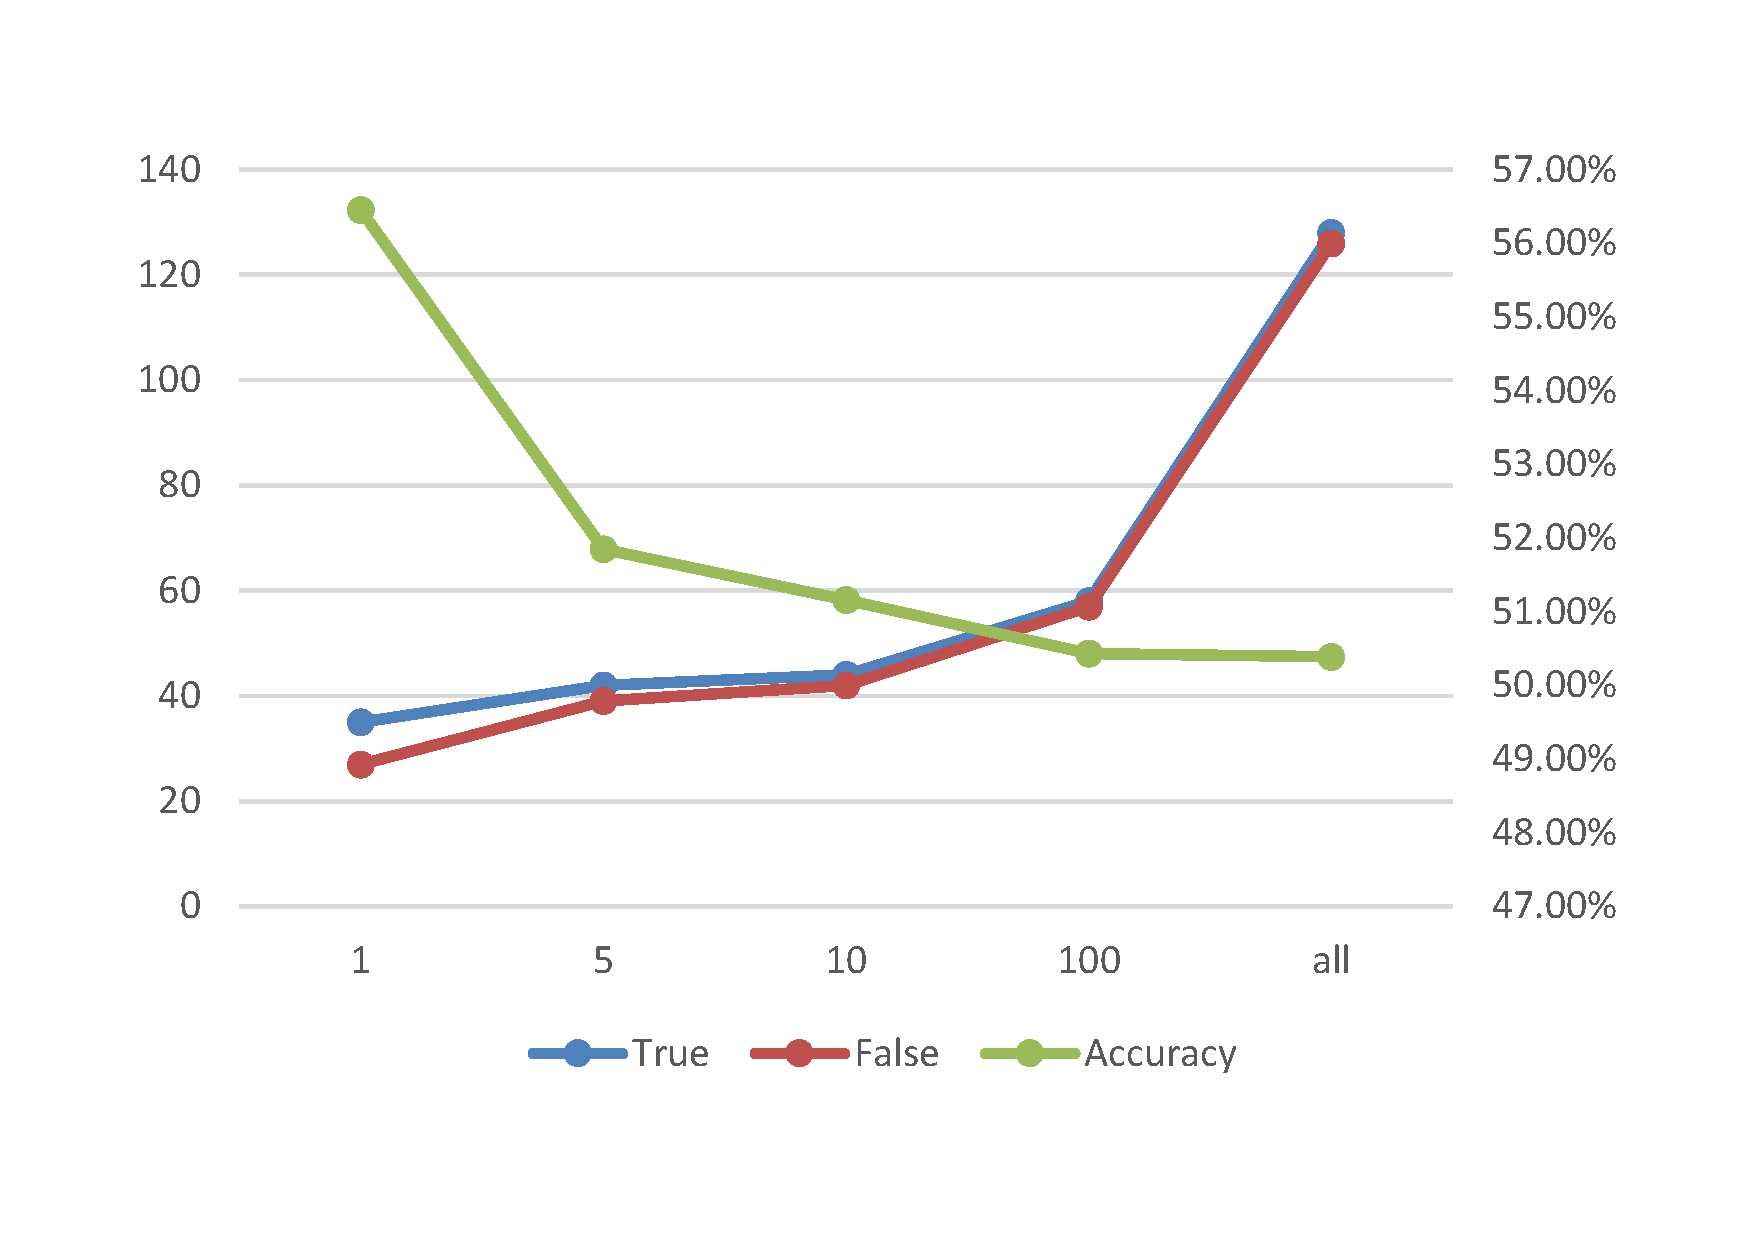
\includegraphics[width=0.9\columnwidth]{figures/rule_futures_prediction}
	\end{center}
	\caption{Futures Price Prediction.}
	\label{fig:futures_price_prediction}
\end{figure}
We choose futures price prediction because the futures are common and concrete things existed in ConceptNet and Probase, such as corn, oil, etc.
%\cite{Ding} is the state-of-the-art stock prediction model(EB\_CNN). We follow similar experimental settings. 
We follow similar experimental settings in \cite{Ding}.
From 2018/1/1 to 2018/11/2, we collect all the headlines and the price change of 15 futures as test data, which include \textbf{851} price change events (The price change of more than 1\% relative to the previous day is an event and we only focus on rise or fall events). 

Baseline models: EB\_CNN model \cite{Ding}, the state of the art model in stock price prediction, uses a deep convolutional neural network to model both short-term and long-term influences of events on stock price movements, and the accuracy of futures prediction is \textbf{54.2\%}. Other models in \cite{Ding}, such as EB\_NN, WB\_CNN, and WB\_NN can achieve \textbf{53.0\%}, \textbf{53.2\%}, and \textbf{53.5\%}, respectively. These accuracies of futures prediction are lower than the accuracies of stock prediction shown in the paper.
It may be because the factors affecting the futures price are far less than the stock price and the futures price is much more stable than the stock price, which makes useful training information about the futures less and further affects the accuracy of the models.

Our approach: For each actual future price change event , we get the news headlines for the previous month before this event. 
For each news headline, we extract the event, use Prolog to reason based on the rules and external knowledge bases, and get the top K inferred events sorted by the confidence.
We may have m*K inferred events for this event, m is the number of events occurred in this month. 
Here, we select the price change events(rise or fall) of the future in this actual future price change event from m*K events and calculate the weighted sum of their confidences(rise event weights 1 and fall event weights -1). If the sum value is positive, we predict this future price as a rise event, otherwise as a fall event. If get no related events changing the future's price, do not make prediction. We compare this prediction with the actual price change to evaluate the reasoning effect. 
Figure \ref{fig:futures_price_prediction} shows the average prediction result. It shows the more predicted events inferred from the Prolog(by increasing K) we use, the lower the prediction accuracy is(from \textbf{56.5\%} to \textbf{50.4\%}), and the more futures events we can predict(from \textbf{62} to \textbf{254}). 

\textbf{\textit{To sum up}}, our rule-based prediction approach can have a higher prediction accuracy (56.45\%) and better interpretation ability with a low recall rate, which is very practical in life.

%\begin{table}[htbp]
%	\caption{Baselines and Proposed Framework}
%	\begin{center}
%		\begin{tabular}{lll}\hline
%			& Acc & MCC \\\hline
%			WB-NN &  0.535 &     \\
%			WB-CNN&  0.532  &     \\
%			EB-NN &  0.530  &     \\
%			EB-CNN&  0.542   &     \\
%			Rule &     &    \\\hline
%		\end{tabular}
%		\label{tab:baselines_and_rule}
%	\end{center}
%\end{table}

\subsection{Downloading and Demo}
The translated Chinese Probase and ConceptNet and learned rules are available at URL.
We built a demo to demonstrate the reasoning process at URL. 
We also developed an application demo of futures prices change triggering that can monitor news from around the world in real time, find the news that may cause futures prices changes, and alert users. Visit URL.
\section{Related Work}
\paragraph{Clarification Question Generation} The concept of CQ can be naturally raised in a dialogue system where the speech recognition results tend to be erroneous so that we raise CQs for sanity check \citep{stoyanchev2014towards}, or the intents for a task is incomplete or ambiguous in a first short utterance and further CQs are needed to fill in the slots \citep{dhole2020resolving}. The concept is then extended to IR to clarify ambiguous queries \citep{aliannejadi2019asking}, and has been successfully put into practice \citep{zamani2020generating}. Other application areas including KBQA \citep{xu2019asking} and open-domain dialogue systems \citep{aliannejadi2020convai3}. CQGen can also be applied to help refine posts on websites like StackExchange \citep{Kumar_2020} and Amazon \citep{rao2019answer}. In this context, our work closely follows the research line of \citep{rao2018learning, rao2019answer, cao2019controlling}. \citet{rao2018learning} first adopted a retrieval-then-rank approach. They \citep{rao2019answer} then proposed a generation approach to train the model to maximize the utility of the hypothetical answer for the questions with GAN, to better promote specificity. \citet{cao2019controlling} propose to control the specificity by training on data with explicit indicator of specificity, but it requires additional specificity annotation. Towards the similar specificity goal, we adopted a different keyword-based approach. They also assume generating one question per context, which we claim is not sufficient to cover various possible information needs, and thus propose the task of the diverse CQGen.

\paragraph{Diverse Generation} The demand for diverse generation exists in many other fields~\cite{vijayakumar2018diverse, LiangZ18code, shen2019mixture}, and we've drawn inspirations from these literatures. For image captioning, we may use multiple descriptions for different focusing points of a scene. \textit{Diverse Beam Search} \citep{vijayakumar2018diverse} was proposed to broaden the searching space to catch such diversity by dividing groups in decoding and imposing repetition penalty between them. For machine translation, a context can be translated with different styles. \citet{shen2019mixture} thus proposed \textit{Mixture of Expert} models including hMup to reflect various styles with a discrete latent variable (\textit{expert}). And here for CQGen, diversity is required to cover various potentially missing aspects, so we come up with the idea to use keywords as a controlling variable like \textit{expert} to promote diversity.


\section{Conclusion}

In this paper, we incorporated the idea of Cookie Theft picture description task into the evaluation of the high-level cognitive abilities of LVLMs and designed a novel evaluation benchmark called CogBench.
% Images in CogBench are of high quality and require more cognitive reasonings to understand, which makes it different from existing image datasets.
The images in CogBench are of high quality and demand more complex cognitive reasoning for interpretation, setting it apart from existing image datasets.
% It consists of a image description task and a VQA task.
Experiments show that there is still a large gap between the cognitive abilities of LVLMs and human beings, indicating CogBench is a challenging benchmark.

% In the future


\bibliographystyle{abbrvnat}
{\renewcommand{\baselinestretch}{0.90}
\normalsize
\bibliography{ocp,gcc}
}
\end{document}
